\documentclass{article}

\usepackage{amsmath,amssymb}
\usepackage{fullpage}
\usepackage[dvipdf]{graphicx}
\usepackage[svgnames]{xcolor}
\DeclareGraphicsExtensions{.pdf,.jpeg,.png}
\usepackage{threeparttable}

\newcommand{\lstfontfamily}{\ttfamily}
\usepackage{listings}
\lstset{%listings package
  language=c++,
  basicstyle=\lstfontfamily,
  emphstyle=\color{red}\bfseries, 
  keywordstyle=\color{DarkViolet}\bfseries,
  commentstyle=\color{DarkGreen},
  stringstyle=\color{DarkBlue},
  numberstyle=\color{DarkGrey}\lstfontfamily,
  emphstyle=\color{red},
  % get also javadoc style comments
  morecomment=[s][\color{Maroon}]{/**}{*/},
  % morekeywords=[1]{include},
  columns=fullflexible,
  % escapeinside=`',
  % escapechar=@,
  % convenience commands, anything between a pair of @@ is in blue color
  moredelim=**[is][\color{blue}]{@}{@},
  showstringspaces=false,
  escapeinside={(*}{*)},
  numbers=left}

\lstdefinelanguage{plain}{
  keywords={}}

\usepackage{enumitem}

\newlength{\mylen}
\AtBeginDocument{\setlength{\mylen}{\fontcharht\font`X}}
\newcommand\cbox[1][black]{\textcolor{#1}{\rule{\mylen}{\mylen}}}

%\usepackage{dirtree}
\usepackage{forest}

\begin{document}

\title{The Loci Multithreading System}

\author{Yang Zhang}

\maketitle

This document details the current (2016) design and implementation of
the multithreading system and related supporting infrastructure in the
Loci framework.  It provides documentation support for future developers
of the Loci system wishing to understand, extend, and maintain the
multithreading modules.  Such developers are also encouraged to read
through the related source files in the Loci code base, as those files
contain additional comments and information pertaining to the
implementation and coding considerations of the multithreading system.
Relevant source files will be outlined later in this document.

\section{Overview}
The main goal of the multithreading modules is to extend the Loci
framework to better support next generation high performance computing
systems.  The Loci framework already supports distributed memory and
runs well on pure distributed memory systems.  It however lacks support
of multithreading scheduling and code generation, making it less than
ideal to run on mixed distributed and shared memory systems, which is
the main architecture employed today.  The multithreading system adds
the thread level parallelism to the Loci framework, making it able to
exploit a hybrid form of parallelism consisting of MPI and threads.
When both enabled, Loci applications will be first distributed to MPI
processes and then further partitioned to multiple threads within a
single MPI process.  The initiation of the multithreading system will
also hopefully  pave the way for future enhancements to the system such
as addressing the vector parallelism paradigm that is also on the rise
in recent time.

The Loci multithreading system has been tested and verified using the
Chem test suite.  Although it is considered ready for real production
use, there has not been large-scale production run using the
multithreading system.  Future developers may need to perform careful
studies and evaluations of the multithreading system to observe its
behavior for large-scale real-world problems.

Also preliminary performance testing and evaluation has been conducted
for the multithreading system.  In the preliminary evaluation, it has
been found that the multithreading system is generally effective, though
its raw peak performance cannot compete equally well with a pure MPI
parallelism.  Much work has been conducted to try to identify the
performance bottleneck in the multithreading system.  Although there is
currently no definitive conclusion to this question (due to the
complexity and nature of non-trivial multithreading programs), the most
plausible cause seems to be the data locality issues.  There are also
several current Loci internal designs that may also degrade threading
performance.  Another issue is that current performance evaluation has
been carried out on relative small-scale (up to dozens of threads).  The
performance behavior of the multithreading system under large-scale
thread parallelism (e.g., up to hundreds or thousands of threads) is
unknown.  This document together with the comments in the source code
will try to point out several important issues that may be affecting the
threading performance.

During the design and development of the Loci multithreading system,
several new thoughts and ideas have also emerged.  Some of these relate
mainly to the multithreading system itself (but was not implemented due
to current software architecture constraints or lack of time), while
several others offer potential improvements to the Loci system in
general.  This document will also try to point out some of these
thoughts so that future developers may consider to adopt/adapt some of
them in the Loci system as it continues to evolve.

\section{Installation, setup, and source code organization}
The multithreading modules are fully integrated within the Loci
framework.  There is no separate installation requirement.  Once the
Loci framework is installed, the multithreading modules are also
installed.  By default, the multithreading functionality is not enabled.
To compile the multithreading code into the Loci library, the
\texttt{PTHREADS} macro has to be defined for the compiler to see, and
the \texttt{pthread} library needs to be linked to the object code.
Since the current Loci installation uses configuration files, it is
suggested to add the following section into the file \texttt{sys.conf}.
And then add these macro definitions to the relevant sections in the
\texttt{comp.conf} and \texttt{sys.conf} files.  In the future, when the
multithreading system is deemed sufficiently robust, it may be compiled
into the Loci framework by default by removing these requirements.

%\noindent\rule{0.85\textwidth}{0.4pt}
\begin{verbatim}
        #########################
        THREADS = -DPTHREADS
        THREAD_LIB = -lpthread
        THREAD_INCLUDE =
        #########################
\end{verbatim}
%\noindent\rule{0.85\textwidth}{0.4pt}

Figure \ref{fig:src-overview} is a diagram of the organization of the
main source code files containing the implementation of the
multithreading modules within the current Loci code base.  The brief
comments within the parentheses provide a summary of the main purpose of
that particular source code file in the multithreading implementation.
The most important files are \texttt{thread.h} and
\texttt{thread.cc}.  These files are specifically created from scratch
and contain the overall architecture and major scheduling and execution
mechanisms of the multithreading system.  All other related files
mentioned in Figure \ref{fig:src-overview} contain specific patches and
enhancements to previous codes that support multithreading
functionality.  These patches and enhancements can be roughly sorted
into the following categories:
\begin{itemize}
  \item Fix of existing code so that thread safety issues are not
    violated.  Most of the fixes occur in the original event dispatch
    code.  
  \item Enhancements made specifically to improve multithreading
    function and performance.  These mainly include removing thread
    blocking requirements in some of the container classes (see section
    \ref{sec:hiddensync} for more discussion), and changes to the rule
    kernel executions to better suit multithreading.
  \item Patches made to each rule compiler and execution module so that
    a special multithreaded module will be compiled and generated when
    multithreading is enabled.  For example, the file
    \texttt{comp\_chomp.cc} contains chomping related modules that
    generate Loci execution back-end for chomping scheduling.  In the
    multithreaded version, it also includes code that determines when
    and how to generate multithreaded versions of chomping scheduling.
  \item Changes made to the Loci scheduler to incorporate multithreading
    scheduling.
\end{itemize}

\begin{figure}%[h]
  \begin{center}
    \begin{forest}
      for tree={
	font=\ttfamily,
	grow'=0,
	child anchor=west,
	parent anchor=south,
	anchor=west,
	calign=first,
	edge path={
	  \noexpand\path [draw, \forestoption{edge}]
	  (!u.south west) +(7.5pt,0) |- node[fill,inner sep=1.25pt] {} (.child anchor)\forestoption{edge label};},
	  before typesetting nodes={
	    if n=1
	    {insert before={[,phantom]}}
	    {}
	  },
	  fit=band,
	  %s sep=2pt,
	  before computing xy={l=15pt},
	}
	[src/
	  [include/
	    [Tools/
	      [cptr.h (thread safety fix)]
	      [Handle.h (thread safety fix)]
	      [lmutex.h (thread safety fix)]
	    ]
	    [execute.h (threading/non-threading rule kernel interface)]
	    [rule.h (threading/non-threading rule kernel interface)]
	    [parameter\_def.h (non-blocking fast\_copy)]
	    [parameter\_impl.h (non-blocking fast\_copy)]
	    [store\_rep.h (non-blocking fast\_copy)]
	  ]
	  [Tools/
	    [eventNotify.cc (thread safety fix)]
	  ]
	  [System/
	    [thread.h (main impl)]
	    [thread.cc (main impl)]
	    [comp\_chomp.cc (chomping rule related changes)]
	    [comp\_impl.cc (pointwise rule related changes)]
	    [comp\_recurse.cc (recursive rule related changes)]
	    [comp\_reduce.cc (reduction rule related changes)]
	    [comp\_tools.cc (misc changes)]
	    [Initialize.cc (scheduler related changes)]
	    [rule.cc (threading/non-threading rule kernel interface)]
	    [sched\_comp.cc (scheduler related changes)]
	    [sched\_tools.h (threading/non-threading rule kernel interface)]
	    [scheduler.cc (scheduler related changes)]
	    [store\_rep.cc (non-blocking fast\_copy)]
	  ]
	]
    \end{forest}
    \caption{Loci multithreading implementation source code organization\label{fig:src-overview}}
  \end{center}
\end{figure}

If multithreading support is compiled into the Loci framework, it can be
activated using the command-line switch ``\texttt{--threads}.''  For
example, suppose ``\texttt{app}'' is the name of a Loci application,
then issuing the command: \texttt{app --threads 8} will launch the
\texttt{app} program using eight threads.  If the option
``\texttt{--threads}'' is not provided, then the program will only run
in a single thread (the default one in a process).  Currently a maximum
of 24 threads may be used within a single application process.  If in
the future, large-scale thread parallelism performance is proved to be
sufficiently good, then this limit can be removed (in file
\texttt{scheduler.cc}).  Issuing the command:
\texttt{mpirun -np 4 ./app --threads 8} will launch the program
\texttt{app} using four MPI processes (working in parallel) and eight
threads within each MPI process (for a total parallelism of 32 execution
units).  In addition, the following command-line options are also
provided to fine tune multithreading behavior:

\begin{itemize}
  \item \texttt{--thread\_blocks <n>}, where \texttt{n} is a number used
    to provide maximum blocks to be used within a single thread.  See
    section \ref{sec:rule-impl} for discussions of thread blocking.  If
    this option is not provided, then a default value of ten is used.
    The current maximum value of the \texttt{n} that can be used is 99.
  \item \texttt{--no\_threading\_pointwise}.  If provided, then all of
    the Loci pointwise rules will not be scheduled using multithreading.
  \item \texttt{--no\_threading\_global\_reduction}.  If provided, then
    all of the Loci global reduction rules will not be scheduled using
    multithreading.
  \item \texttt{--no\_threading\_local\_reduction}.  If provided, then
    all of the Loci local reduction rules will not be scheduled using
    multithreading.
  \item \texttt{--no\_threading\_chomp}.  If provided, then all of the
    Loci chomping rules will not be scheduled using multithreading.
  \item \texttt{--no\_threading\_recursion}.  If provided, then all of
    the Loci recursive rules will not be scheduled using multithreading.
\end{itemize}

\section{Overall design considerations}
This section discusses the overall design choices and considerations
related to high-level multithreading facility.  First of all, the
multithreading modules continue to use data parallelism in the same way
as the existing distributed memory implementation.

Figure \ref{fig:loci-overview} shows the task and data parallel view of
multithreading execution of a set of Loci rules.  Task parallelism
assigns entire rule computation to different threads, while data
parallelism assigns sub-domains in each rule to different threads.
These are the two major forms of thread level parallelization strategies
in use today.  In all of current Loci applications, the task parallelism
level is quite small since there will only be a small set of independent
rules at a given scheduling step.  Therefore in the current
implementation, data parallelism is used since the domain of each rule
is usually very large.  And therefore data parallelism supports a much
larger thread level concurrency.  It is possible to mix the two forms of
thread level parallelism in the Loci framework and it may provide some
benefits for certain types of applications.  This is left as a future
improvements.  At the present time, only data parallelism is beneficial
to any multithreading scheduling of Loci applications.

\begin{figure}[h]
  \begin{center}
    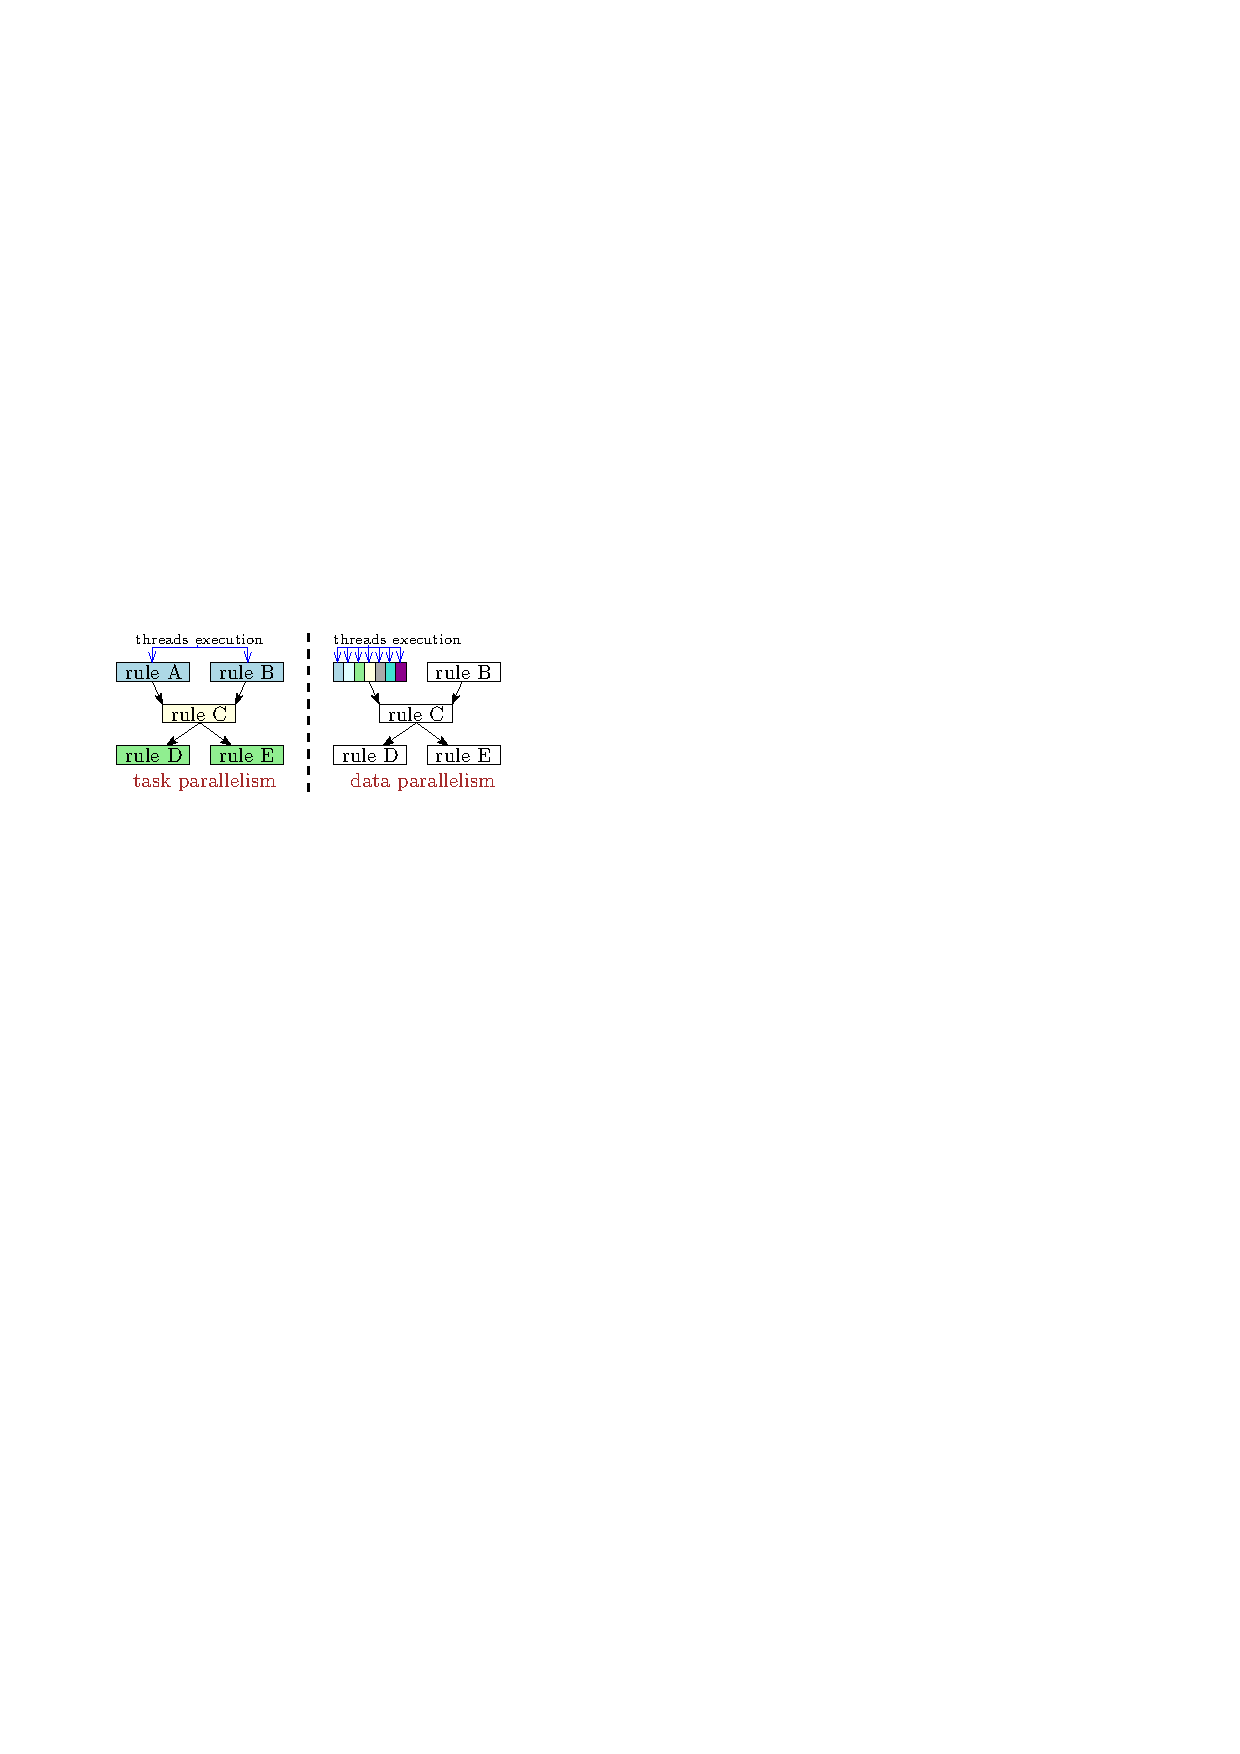
\includegraphics[width=0.75\textwidth]{loci-overview}
    \caption{Task and data parallelism\label{fig:loci-overview}}
  \end{center}
\end{figure}

Another issue is load balancing.  We do not perform any dynamic load
balancing to the current multithreading schedules.  The reason is the
same as we do not have dynamic load balancing in the current distributed
memory schedules --- the cost of computation kernel applied to each
entity in a rule domain is usually uniform.  Load balancing is another
reason why we have only adopted the data parallelism form for
multithreading schedules.  The task parallelism would usually require
some form of dynamic load balancing to distribute the work evenly to all
threads as the cost of different rule computations may indeed be
dramatically different.

In recent development of multithreading programming, an important class
of technique called ``logic parallelism'' is increasingly gaining
widespread adoption.  Representative languages and systems that use such
concurrency paradigm include the Intel Cilk and Threading Building
Blocks, the Java executer and fork/join frameworks, as well as a number
of other research products.  Systems using logic parallelism employ a
scheduling layer that sits between the program specification and the
machine hardware.  In the program specification, the programmer uses
language and system constructs to indicate at a high level where
parallelism {\em might} occur, and/or where executions {\em can} happen
concurrently.  These special constructs provide the middle layer hints
how and where parallel execution can be scheduled and they usually also
support recursive and nested logic parallelism.  In the logic view of
the program, the total number of threads can be unbounded.  The middle
layer then schedules these logic threads onto a given set of low level
system threads (such as real hardware threads or threads provided by
certain libraries).  The scheduler can usually also be configured in
different ways and works transparently in the background from the
programmer's perspective.  Several such systems also employ provably
optimal scheduling policies that generate asymptotically guaranteed
thread scheduling performance.

The Loci framework can also be structured to take advantage of such
logic parallelism.  For example, all the entities that form the
domain of a Loci rule can be partitioned into large numbers of small
chunks each contains a few (maybe on the order a few dozens) entities.
Then each such chunk together with the computational kernel can be
treated as a ``logic'' task and handed over to the thread scheduler.
The runtime thread scheduler will take care of the mapping, scheduling,
and load balancing issues.  Another way to restructure a Loci rule
computation would be to split the rule domain in half recursively and
let the system scheduler deal with the management of nested parallelism
on a fixed number of hardware threads.  Using such an approach can
dramatically simplify taking advantage of multithreading concurrency as
the middle layer scheduler takes care of vast number of important issues
automatically.  It also provides a means of dynamic load balance within
the participating threads.  Loci rules under this paradigm will only be
viewed as collections of small chunks and each chunk is computed
independently.  So long as the dependency that produces correct results
is respected, the scheduler is free to mix and reorder the execution of
all these chunks as it sees fit.

However we have decided to not adopt such ``logic parallelism'' in our
implementation of multithreading in Loci.  The first reason is that this
will add dependency and make the Loci code base rely on more external
libraries and packages, whose future status and standard comformance
plans are not entirely clear.  We want to maintain as minimal dependence
as possible and as much standard compliant as possible.  The more
important reason is that these logic threading parallel programming
libraries, while increasingly being adopted, are mainly targeting
application development.  We have a unique situation where we ourselves
are developing a runtime system and programming tools (and not
application level software).  Thus if we employ some of these libraries
to do multithreading, we will lose some opportunities to customize and
optimize the code for our own case.  Loci can be viewed as on the same
abstraction level as those logic threading parallel libraries.  Thus
essentially we would want to develop our own equivalent version of those
parallel libraries.  Doing so also provides us chances where we can take
advantage of special Loci features to better support its applications.

Another notable recent development is the modern C++ standard (c++11 and
c++14, and the upcoming c++17).  These are quite major updates to the
C++ language.  The current standard also added multithreading support
as standard libraries in the \texttt{std} namespace.  In terms of c++11
threads support, there are three main components. The first is
essentially the same mechanism as the older POSIX-thread programming
mechanism, wrapped in nicer C++ constructs.
The second part is the support of
asynchronous programming through the \texttt{std::future},
\texttt{std::promise}, and \texttt{std::packaged\_task}
mechanism.\footnote{It would be nice to have these constructs support
  the logic parallelism discussed early.  They appear to be mostly
  mirroring similar constructs and mechanisms on the Java platform.
  Unfortunately at this writing, these new c++11 constructs do not (yet)
  support true logic parallelism.  The current C++ thread implementation
  does not appear to use a sophisticated thread scheduler to support
  dynamic thread scheduling.  We would hope however, that implementations
  in the future would catch up to provide true logic parallelism and 
  dynamic threading support.}  The third part is the addition of a set
of atomic variables and an associated memory model that guarantees
sequential consistency behavior if certain rules are followed.

Since Loci was developed in C++, this will have a major impact on how we
actually implement our multithreading infrastructure.  We have not
adopted in using modern C++ so far.  One major reason is that the
adoption relies on all our clients willing to upgrade to the newest C++
compiler and libraries.  Fully upgrading Loci framework to modern C++
probably also means that some of the previous code will break and it
will take time to fix everything.  Secondly, for the same reason that we
are not developing application level software means that we are less
dependent on many features.  For example, so far we do not need the
asynchronous threading support from the new C++ thread library.  However
we would stress that although we did not incorporate modern C++ into
the current Loci multithreading infrastructure, moving towards the
adoption of it is inevitable.  Fully employ the modern C++ facility in
the near future is advised.  This has the benefit of staying current and
relevant to the programming language we use.  In addition, several C++
threads features (such as the atomic variable and standardized memory
semantics) will be very helpful as well to support our development.

\section{Thread architecture design and implementation}
\label{sec:design}
This section provides discussions on the high level implementation of
the current Loci multithreading modules.  It outlines the major
algorithms in use in the multithreading system.  The Loci code base
contains additional comments about actual code that implements these
algorithms.  A major goal of this development is to keep the public
interface of the Loci framework the same as before. In this way, users
and all existing Loci programs do not have to make any significant
changes to utilize the new threads capability.  Currently the new
threads implementation follows the same Loci software architecture and
is made to be extensible.  


\subsection{Overall software architecture}
\label{sec:tm}
Since we schedule and manage low level threads in the Loci framework,
the top-level and most important software architecture in our threads
infrastructure is the ability to generate and manage threads.  For this
purpose, we designed an interface for such requirements.

\begin{figure}[h]
\begin{lstlisting}
// in file "src/System/thread.h"
class ThreadControl {
public:
  virtual void create_threads() = 0;
  virtual void shutdown() = 0;
  virtual void restart(vector<@ThreadedExecutionModule@>&) = 0;
  virtual void wait_threads() = 0;
};
\end{lstlisting}
\caption{The abstract thread manager\label{fig:tm}}
\end{figure}

The \lstinline{ThreadControl} type serves as a required interface that
the thread manager in Loci should be able to support (only partial
interface shown in Figure \ref{fig:tm}).  This essentially models a
thread pool, where low level threads are not created and destroyed as
the lifetime of the tasks put on them.  Instead, a fixed number of
low level threads are created and reused all the time for all
computations in the system.  The reason is clear because creation and
destruction of low level threads are generally expensive.  We want to
reuse a low level thread whenever possible.

There are two types of threads in the system, the main control thread
and the work threads.  There is only one control thread in the system
and it is created by the process.  There can be multiple work
threads existing at the same time.  Work threads are all created by the
main control thread.  The control thread only invokes
methods defined in the \lstinline{ThreadControl} type and does not
participate in any computation.  The work threads are managed by the
control thread and they only participate in actual computation.

The \lstinline{create_threads()} method will create all the low level
threads necessary (the exact number is defined at the construction time
of a concrete thread manager).  After creation, each thread will be in a
suspended state waiting for any work to come.

The \lstinline{shutdown()} method terminates all created low level
threads. And the \lstinline{restart()} procedure will restart all
suspended threads, feeding each with a new work.  The type
\lstinline{ThreadedExecutionModule} defines what a thread work is
(to be explained later in section \ref{sec:int}).

Work threads do not automatically go away after finishing their
assigned work.  They just become inactive.  All the work threads are
explicitly created and destroyed by the \lstinline{create_threads()} and
the \lstinline{shutdown()} calls from the main control thread.

The \lstinline{wait_threads()} causes the main control thread to suspend
waiting for all the active work threads to finish their current
work and then it wakes up.  This also implies that after this function
returns, all work threads will be in a suspended state.

Such a thread control also includes implicit synchronizations among
all the work threads, i.e., all active work threads will
implicitly synchronize after each \lstinline{restart()} call (when they
finish all assigned work in the current step, typically a rule).  See
section \ref{sec:sync} for a discussion how this is implemented.  This
form of bulk synchronization is the same mechanism used in the current
MPI implementation of the distributed memory parallelism (since both are
a form of data parallelism).  It is unclear at this moment whether
removing or relaxing some of the barriers will enhance the performance.
For example, if it is determined that two sequential
\lstinline{restart()}s do not share dependency, then we might be able to
remove the barrier between the \lstinline{restart()}s.  But since we
package entity sets to be handed to work threads, we can equally
create a new task that combines computations in multiple Loci rules and
feed it to the threads.  This is equivalent to removing the implicit
synchronization between rules.  This is an overall complicated
optimization problem, whose solution may require extensive evaluation.

\begin{figure}[h]
  \begin{lstlisting}
// in file "src/System/thread.h"
class ThreadControl_pthread: public ThreadControl {
public:
  void create_threads() { pthread_create(/* ... implementation */) }
  // ... other implementations
private:
  // ... details
};
  \end{lstlisting}
  \caption{A concrete thread manager\label{fig:tm-pthread}}
\end{figure}

We currently use POSIX-threads as our underlying low level thread
generator. We have implemented a concrete thread manager that
instantiates the abstract interface as presented in Figure
\ref{fig:tm-pthread}.  Other threading mechanism can also be packaged as
similar concrete classes that will allow easy switch of the underlying
threading choice (for example, one can also implement a
\lstinline{ThreadControl_cpp} to use the thread library from the c++11
standard as an implementation).

\sloppy{%
In the file \texttt{src/System/thread.cc}, there is a global variable
\lstinline{thread_control} (whose type is \lstinline{ThreadControl*}, a
pointer to the \lstinline{ThreadControl} type).  This global variable
should point to a concrete thread controller that is initialized in the
file \texttt{src/System/sched\_comp.cc}.  Currently if multithreading is
enabled for an application, the global variable
\lstinline{thread_control} is initialized with a
\lstinline{ThreadControl_pthread} object.}

The file \texttt{src/System/thread.h} also contains two classes
\lstinline{StartThreads} and \lstinline{ShutDownThreads}.  They are
subtypes of the Loci \lstinline{execute_modules} type (whose respective
\lstinline{execute()} method invokes the corresponding
\lstinline{ThreadControl} interfaces, \lstinline{create_threads()} and
\lstinline{shutdown()}) and are used to
start and shut down the thread controller (pointed to by the global
variable \lstinline{thread_control}).  These execution modules are
inserted into the overall Loci execution list in the file
\texttt{src/System/sched\_comp.cc}.

\subsection{Integrating threads into existing software architecture}
\label{sec:int}
The current Loci framework compiles each rule specification into a
functional block (called ``compiler'' in the Loci code base).  All of
these functional blocks are then arranged in a linear order as a list
(``scheduling'').  Finally each of these functional blocks in the list is
then converted into an execution module, which is an abstract type with
an \lstinline{execute()} interface that can be called to carry out the
original rule's specification when supplied with a set of entities (the
``context'') and a place to read/write the data associated with the
rule's definition (usually the \lstinline{fact_db}).  

For example, a
Loci \lstinline{pointwise} rule is usually converted into an
\lstinline{impl_compiler} object, which when called, generates the
execution context (represented as a Loci sequence) for the corresponding
\lstinline{pointwise} rule.  The \lstinline{impl_compiler} object is
then linearized in a list of similar compilers objects and eventually
converted to an \lstinline{execute_rule} object, whose
\lstinline{execute()} interface when invoked, finds the rule context and
applies the \lstinline{pointwise} kernel to the context and stores the
associated data in the Loci \lstinline{fact_db}.  This is the main
architecture and mechanism of the Loci framework scheduling.

The multithread implementation reuses such an organization.  When we
detect multithreading is enabled, for each functional block in the
scheduling list where threads can be applied, we will create a special
multithreaded execution module instead of a conventional execution module.
Such special multithreaded execution module is also a subtype of the
common abstract \lstinline{execute_modules} type.  When the
\lstinline{execute()} interface of such multithreaded execution module
is called, it applies the corresponding rule kernel over the entire
computation context using multiple threads (instead of a single thread
as in the conventional schedule).  For example, for a Loci
\lstinline{pointwise} rule and its associated \lstinline{impl_compiler},
instead of producing an \lstinline{execute_rule} object, the
multithreading code produces a \lstinline{Threaded_execute_rule} object,
which is also a subtype of the \lstinline{execute_modules} type.
Figure \ref{fig:texe} shows how a \lstinline{Threaded_execute_rule}
type is implemented in the current Loci base.

\begin{figure}[h]
  \begin{lstlisting}
// simplified impl of Threaded_execute_rule, full version in file src/System/thread.h
class Threaded_execute_rule: public execute_modules {
public:
  Threaded_execute_rule(kernel k, Context c, Storage s) // construction
  { // thread_control is a ThreadControl*, see section (*\color{DarkGreen}{\ref{sec:tm}}*) for details
    p = thread_control->num_threads(); 
    // partition the context into p parts, where p is the number of work threads
    partition = partition_context(c, p);
    for(i=0; i<p; ++i)
      tw.push_back(new @ThreadWork@(k, partition[i], s));    
  }
  void execute()
  {
    thread_control->restart(tw);
    thread_control->wait_threads();
  }
private:
  vector<ThreadedExecutionModule> tw;
};
// ......
// we would replace any of the following code:
return new execute_rule(k,c,s);
// with the following code:
if(multithreading_is_enabled)
  return new Threaded_execute_rule(k,c,s);
else
  return new execute_rule(k,c,s);
  \end{lstlisting}
  \caption{Simplified version of a multithreaded execution module\label{fig:texe}}
\end{figure}

The \lstinline{ThreadWork} in Figure \ref{fig:texe} is a concrete
implementation of the type \lstinline{ThreadedExecutionModule} mentioned
in section \ref{sec:tm}.  This abstract type represents a unit of
workload to be executed on a work thread managed by the thread
controller.  It also mandates an \lstinline{execute()} interface that
accepts a Loci \lstinline{fact_db} and a \lstinline{sched_db} as input
parameters.  These two parameters are not used in most current
implementations.  However they are supplied since the conventional Loci
\lstinline{execute()} interface in the \lstinline{execute_modules}
requires them and they may be used in the future.  A concrete
implementation of the \lstinline{ThreadedExecutionModule} may simply
execute its workload independently, or does some special internal
processing on each different thread, or may require collective
synchronization with other work threads.  Such a detail is determined
solely by the individual implementation.  The multithreaded version of
the \lstinline{execute_modules} only generates and passes a
\lstinline{vector} of such \lstinline{ThreadedExecutionModule} to the
thread controller.  Section \ref{sec:rule-impl} contains more
information on how concrete \lstinline{ThreadedExecutionModule}s are
implemented for different types of Loci rule computations.

\subsection{Thread synchronization}
\label{sec:sync}
The thread controller (\lstinline{ThreadControl}) also implements most
of the thread synchronization operations.  In the current
implementation, all thread synchronizations are distributed, i.e., there
is no global lock and memory space that is accessed by all the threads
in the system. Also in order to reduce the cost of thread context
switch, all locks used in the implementation are spin lock (a spin lock
does not put a blocking thread into a suspended state, two context
switches will occur if a thread goes into sleep and wakes up later).
Since we use distributed locking mechanism and each lock is typically
only shared between two threads, we anticipate the cost of spinning is
small.  The only place where threads are blocked is when all work
threads finish computing a Loci rule.  In that case, we put all work
threads in a suspended state and transfer the control to the main
control thread.  When any of the work threads is active, the main
control thread is suspended.  Currently each thread (including the main
control thread) has an associated POSIX semaphore that is used to block
the corresponding thread.  The pthread implementation
\lstinline{ThreadControl_pthread} in file \texttt{src/System/thread.h}
defines the variable \lstinline{main_block} (a \lstinline{sem_t} type)to
be used to regulate the state of the main control thread; and the
variable \lstinline{worker_block} (a \lstinline{vector<sem_t>} type) to
be used to regulate the state of all of the work threads.

\begin{figure}[h]
  \begin{center}
    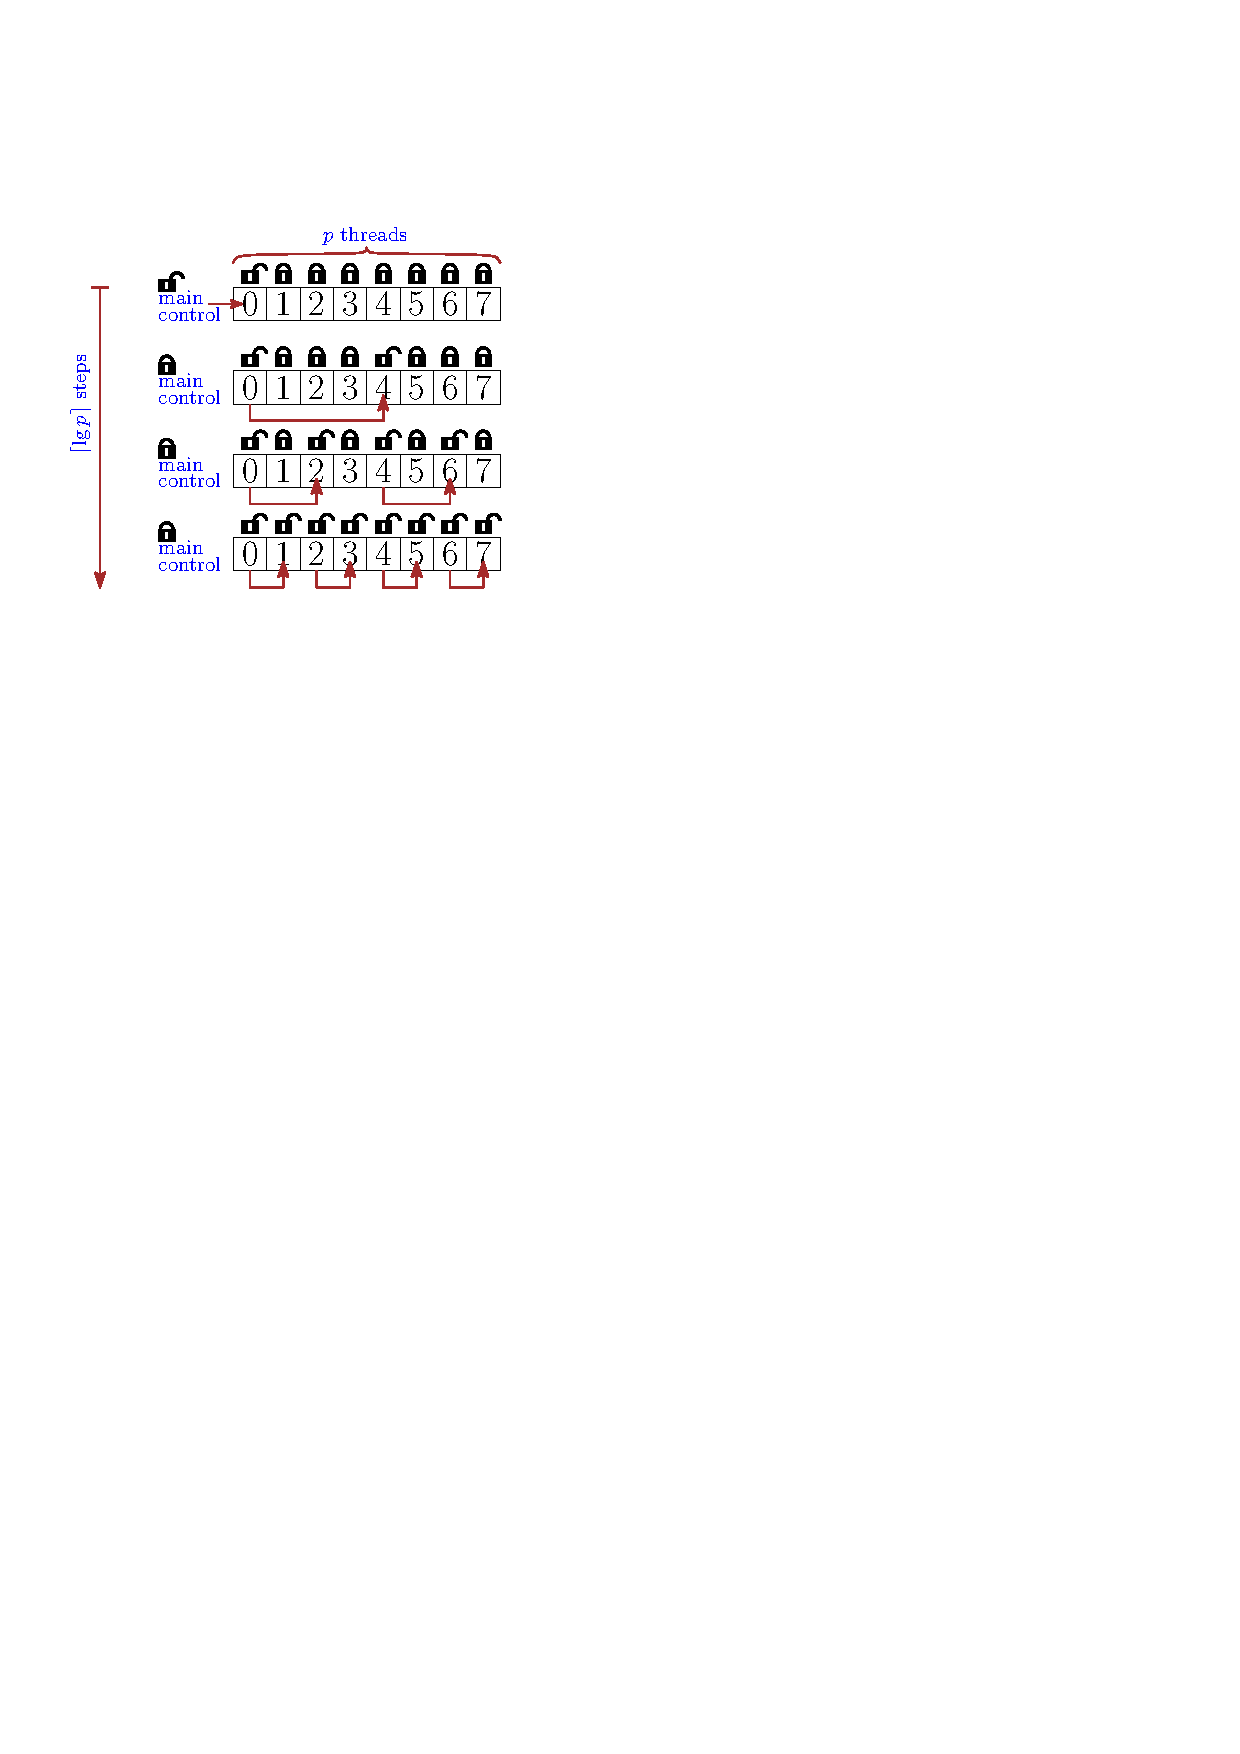
\includegraphics[width=0.5\textwidth]{restart}
    \caption{Thread starting mechanism\label{fig:restart}}
  \end{center}
\end{figure}

The \lstinline{restart} procedure presented in section \ref{sec:tm}
starts all of the work threads from their suspended state and feeds each
one a thread work unit (i.e., \lstinline{ThreadedExecutionModule}).
Figure \ref{fig:restart} illustrates the distributed restarting scheme
used in the current pthread thread controller.  This is a tree based
starting mechanism.  When it is time to start all work threads, the main
control thread unblocks one of the work thread (typically the work
thread with ID 0).  The main control thread is then blocked (by calling
the \lstinline{wait_threads} interface).  Subsequently all of the work
threads are unblocked in a cascading fashion as illustrated in Figure
\ref{fig:restart}.  When the thread controller is constructed, it
computes for each work thread a list of partners to unblock (the
procedure \lstinline{build_partner()} in file
\texttt{src/System/thread.cc}).  For example, thread 0 in Figure
\ref{fig:restart} has the following list: [4,2,1].  There are at most
$\lceil\lg p\rceil$ elements in such a list, where $p$ is the total
number of threads.  Also note that there is no implied synchronization
between the steps in Figure \ref{fig:restart}.  The distributed start
mechanism is completely asynchronous, see Figure \ref{fig:wt} for how
the restart is currently implemented.

\begin{figure}%[h]
  \begin{lstlisting}[escapechar=@]
// full version in ThreadControl_pthread::thread_fun() in file src/System/thread.cc
void work_thread()
{ // block is an array of semaphores indexed by thread id
  // partner is an array of list indexed by thread id, it
  // @\quad@ stores the restart partners for each thread as
  // @\quad@ suggested in Figure @\textcolor{DarkGreen}{\ref{fig:restart}}@
  // tree is an array of list indexed by thread id, it
  // @\quad@ is the static tree barrier shown in the right part
  // @\quad@ in Figure @\textcolor{DarkGreen}{\ref{fig:barrier}}@
  while(true) {
    wait(block[me]); // me represents the id of the calling thread
    for(p : partner[me]) 
      signal(p); // release all partner threads
    // perform thread work by executing the thread work unit explained in section @\textcolor{DarkGreen}{\ref{sec:int}}@
    // thread_work is a vector of ThreadedExecutionModule indexed by thread ID
    thread_work[me]->execute(); 
    // finishing ...
    for(c : tree[me]) {
      done = false;
      while(!done) { // check if child c is done
        spin_lock(c.lock);
        done = c.flag;
        spin_unlock(c.lock);
      }
      c.flag = true; // once child is done, reset its flag
      if(me.parent) { // has a parent node, change local flag
        spin_lock(me.lock);
        me.flag = true;
        spin_unlock(me.lock); // spin locks act as memory fence
      } else // must be the root node
        signal(main); // unblocks the main control thread
    }
  } 
}
  \end{lstlisting}
  \caption{How a work thread functions\label{fig:wt}}
\end{figure}

When all work threads finish computing a Loci rule, the main control
thread needs to be unblocked and continue the subsequent work.  There
needs to be a mechanism to signal that all work threads are done.
This is similar to a barrier design (only that the barrier does not
need to be reusable since we have a separate main control thread that
can perform any reset operation).  A common approach is to use a
global variable initialized to the total number of work threads.  Each
work thread will decrement the counter once it finishes its work.
Whoever decrements the counter down to zero will be responsible to
unblock the main control thread.  This scheme has the potential
disadvantage of causing high memory contention at the location of the
counter variable.

\begin{figure}%[h]
  \begin{center}
    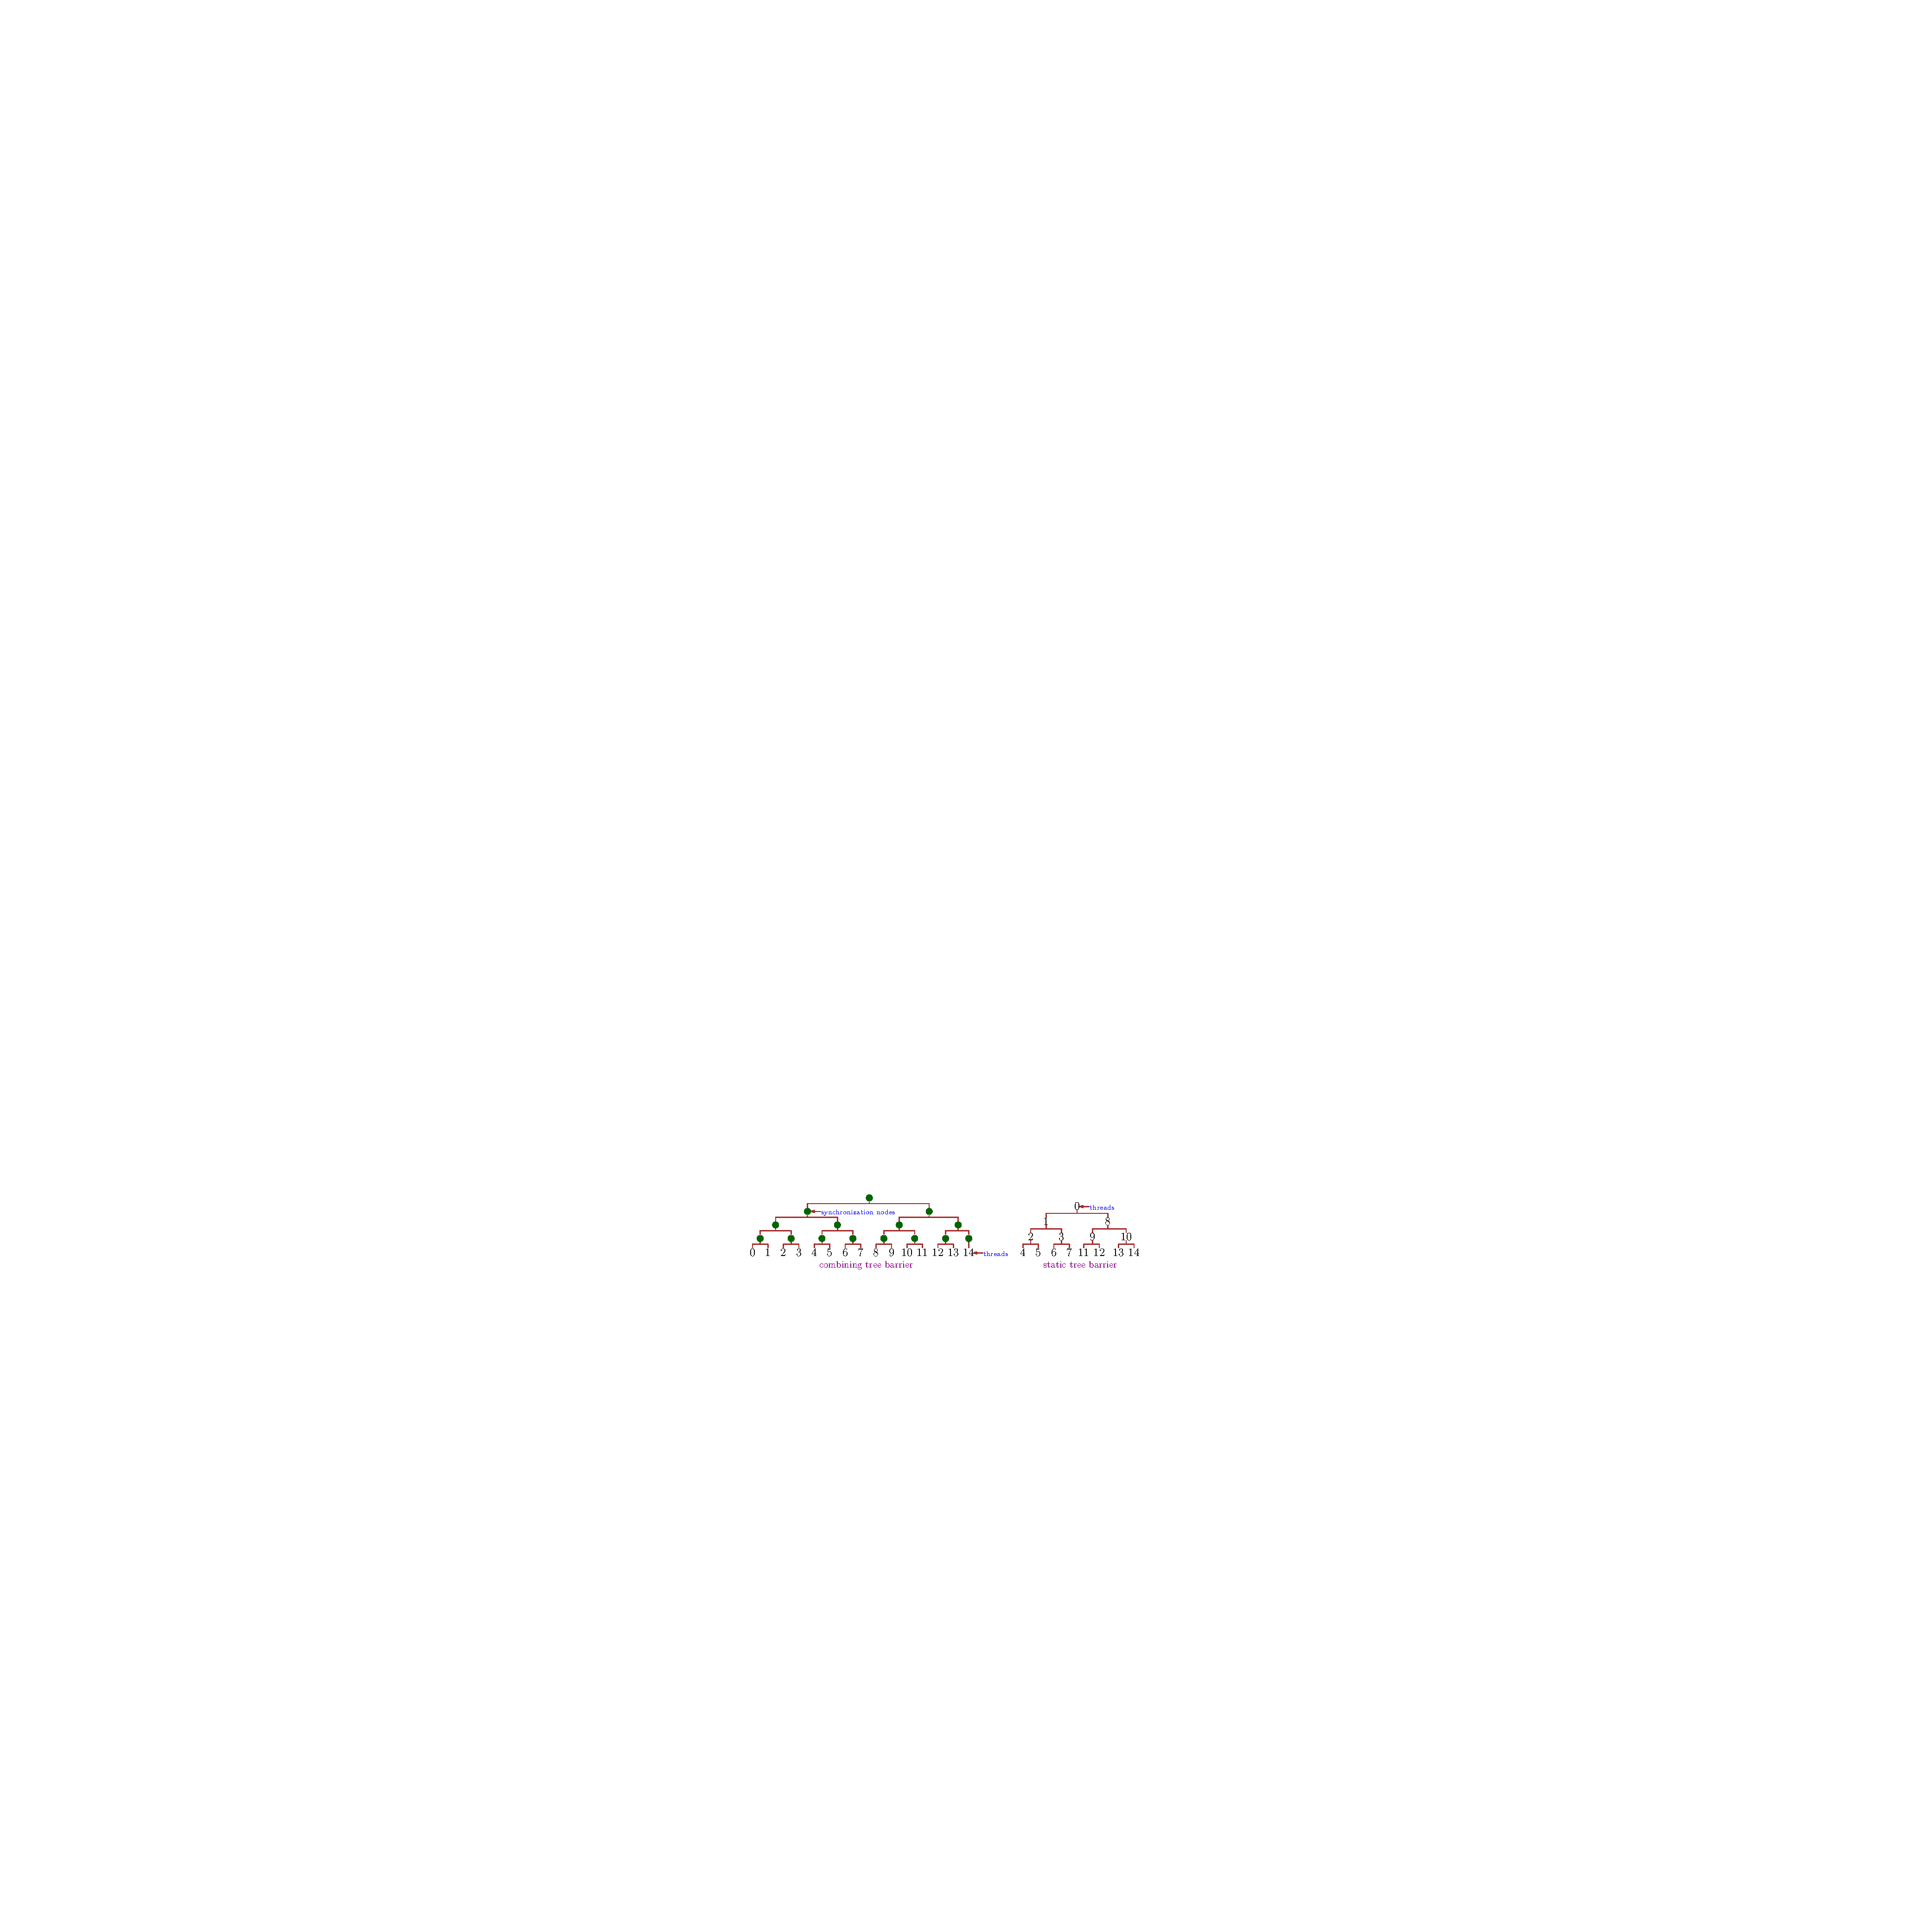
\includegraphics[width=\textwidth]{barrier}
    \caption{Tree based thread suspension\label{fig:barrier}}
  \end{center}
\end{figure}

We have used a tree based distributed barrier design to put all work
threads into suspension and unblock the main control thread.  There
are different ways to implement a tree based barrier.  If we take the
reverse process of the restart as suggested in Figure
\ref{fig:restart}, then we would pair threads as in the left part of
Figure \ref{fig:barrier} (the combining tree barrier).  Each interior
node will be responsible to check the status of its two children.
When all children of a node are done (signaled via spin lock protected
flags), the node then sends the signal upward the tree until the root
node is activated, which then unblocks the main control thread.

Another way is to construct a static tree as suggested in the right
part of Figure \ref{fig:barrier}.  It works almost the same than the
left side tree.  Each thread has at most two children and checks the
status of them upon finishing its own work (also via spin lock
protected flags).  When the root node finds that all of its two
children are done, it then unblocks the main control thread (since
that means everyone is done).  We have adopted this static tree based
distributed barrier mechanism since it constructs a more compact tree
with fewer locks and interactions.  Since the work threads number is
fixed, the thread manager can construct this static tree just once and
reuse it in all subsequent computations (the procedure
\lstinline{build_term_tree()} in file \texttt{src/System/thread.cc}
constructs such a tree).  With all these synchronization mechanisms,
each work thread will run the procedure as shown in Figure \ref{fig:wt}.

\subsection{Multi-level partition}
\label{sec:part}
In order to deal with the complications of thread interactions within a
Loci reduction computation (see section \ref{sec:rule-impl} for
details), a multi-level data partitioning infrastructure was implemented
in the Loci multithreading system.  However this multi-level data
partitioning and the associated scheduling policies in the Loci
multithreading system may not be the best option available.  We have
indeed spent a lot of time trying to come up with different strategies
to design thread scheduling for the Loci reduction rules.  Currently we
think there is a better way to schedule multithreaded reduction
computations in Loci.  Due to lack of time and infrastructure support,
it was not implemented.  Section \ref{sec:arrow} will discuss the main
idea and what's needed to implement it.  However the current multi-level
partitioning based multithreaded reduction works reasonably well in the
Loci system.

The basic idea of the multi-level partition is to extend the data
partitions made for each MPI process and further partition them for each
work thread on an MPI process.  Figure \ref{fig:mltp} shows an example
of such partitioning.  In this example, an input mesh is broken into
three parts for a three-MPI process run.  Each MPI process gets one
piece of the input mesh (details such as ghost regions are omitted in
this example).  Furthermore each MPI process starts two threads.  The
light green colored region in Figure \ref{fig:mltp} shows an instance of
the configuration on one of the MPI processes.  The process owned data
(in magenta) is further partitioned into two subparts.  Each work thread
gets one such part.  Furthermore on each thread, the data is again
partitioned into multiple smaller parts.  Notice that the actual data is
not being duplicated in such partitioning, only the data indices (i.e.,
the entities) are regrouped together.

\begin{figure}[h]
  \begin{center}
    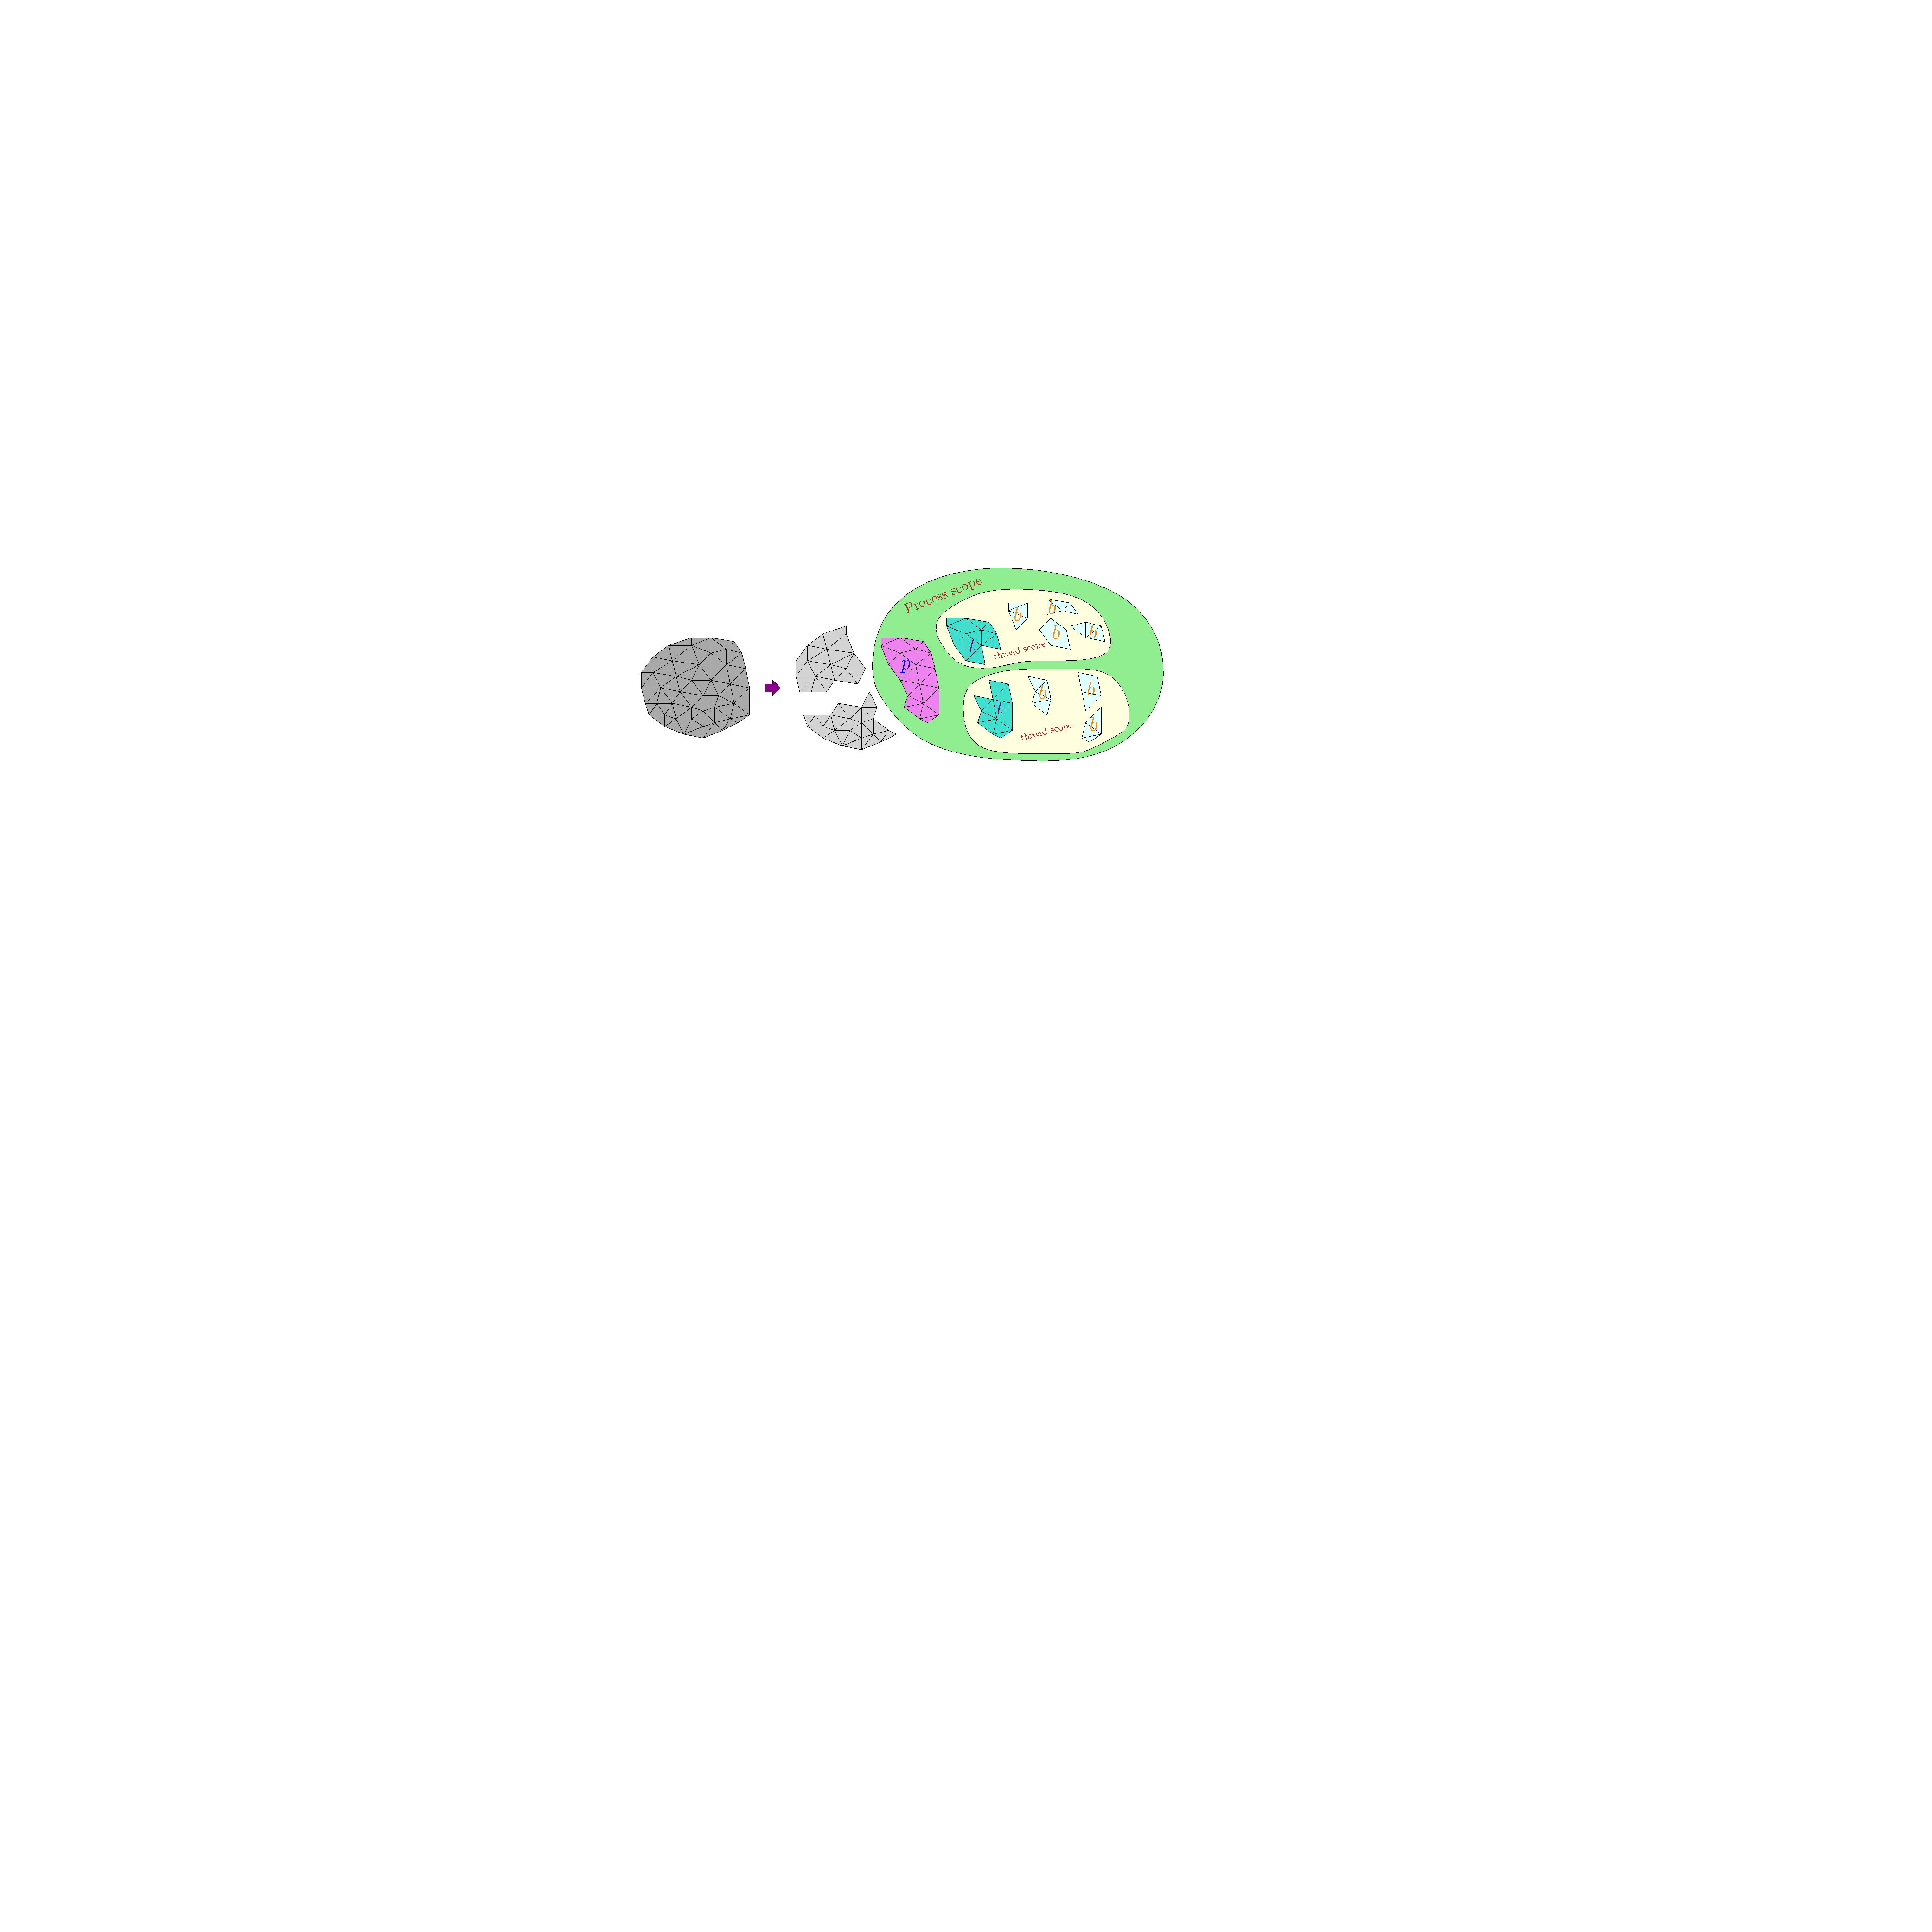
\includegraphics[width=0.85\textwidth]{multi-partition}
    \caption{Multi-level partition overview\label{fig:mltp}}
  \end{center}
\end{figure}

Essentially the entire process consists of a three-level partitioning
and produces a triple ``$(p,t,b)$'' partitioning of the original input
mesh.  In this scheme $p$ stands for the number of MPI processes, $t$
stands for the number of work threads on each process, and $b$ stands
for the number of blocks on each thread.  Thus, the initial mesh is
first partitioned into $p$ parts, then each of these $p$ parts is
partitioned into $t$ parts, and each of the $t$ part is again
partitioned into $b$ parts.  As a result, each process owns one of the
$p$ parts.  Each thread owns one of the $t$ parts as well as all the $b$
parts that form the single $t$ part.  Each of these partitions will try
to balance the number of entities inside.  They will also try to
preserve data locality as much as possible.  This means that all of the
data that stay within a single such partition (no matter on the $p$,
$t$, or $b$ level) are close to each other with respect to the data
access pattern in the application.  However the actual partition
strategy for each of the levels may be different from each other.  

Parallelism is supported within the Loci framework on all of the
$(p,t,b)$ levels.  The $p$ level parallelism is generated by MPI calls
and the $t$ and $b$ level parallelism are exclusive to threads.  Some of
the multithreaded computations will only have parallelism on the $t$
level, while some of the threaded computations will have parallelism on
the $b$ level as well.  Section \ref{sec:rule-impl} will give a detailed
review.  Below the $b$ level, a single computation could decide to
further partition the data to do special processing related to that
particular computation.  However there will be no thread level
parallelism supported below the $b$ level.  Therefore any partition
below the $b$ level is solely managed by individual computation and is
used for purposes other than generating parallelism.

Currently the $p$ level partitioning strategy is handled by the Loci
grid reader (using either a graph or a spatial based algorithm).  The
current $t$ and $b$ level partitioning are directly handled inside the
thread controller object and are based on a spatial partitioning
algorithm on a primary variable and topological affinity with
tie-breaking.  We use an abstract type \lstinline{ThreadPartition} to
define the interfaces that must be supported by any thread-level data
partition implementation.  Figure \ref{fig:tp} shows the important
portion of such an interface.

\begin{figure}[h]
  \begin{lstlisting}
// in file "src/System/thread.h"
struct ThreadPartition {
  virtual void create_thread_domain(fact_db& facts) = 0;
  virtual std::vector<sequence> partition_by_domain(const sequence& s) const = 0;
  virtual std::vector<int> partition_by_blocks(int t, const sequence& s) const = 0;
  virtual sequence refine_seq_by_block(int t, int b, const sequence& s) const = 0;
};
  \end{lstlisting}
  \caption{Thread level partition interfaces\label{fig:tp}}
\end{figure}

The interface \lstinline{create_thread_domain()} is used to generate
within an MPI process, all of the $t$ and $b$ partitions as discussed
above.  This interface is usually invoked by a concrete thread
controller (the current \lstinline{ThreadControl_pthread} calls this
interface during its construction time, see file
\texttt{src/System/thread.cc} for details).  After calls to this
interface, each MPI process should have a data structure containing
information that assigns a given entity to a specific $t$ and $b$
partition.

The interfaces \lstinline{partition_by_domain()} and
\lstinline{partition_by_blocks()} split a given context according to the
$t$ and $b$ partitions respectively.  These two interfaces are primarily
used to split a process-level context into thread-level context.
Section \ref{sec:rule-impl} uses these interfaces to implement
multithreaded scheduling of different Loci rules.

The interface \lstinline{refine_seq_by_block()} generates an accurate
context given a $t$ and $b$ partition index and a rough context.  It is
needed because a rule context may only span part of a block.  For
example, a thread may contain three $b$ level blocks, each containing
several entities: $b_0 = [1,10]$, $b_1 = [11,20]$, $b_2 = [21,30]$ (the
entire domain for the thread is therefore $[1,30]$).  A particular rule
context may be $[5, 25]$ for example.  Then such a context will span
blocks $b_0$, $b_1$, and $b_2$ on this thread.  Such block-level
information is needed during scheduling phase.  But such a context only
spans part of $b_0$ ($[5,10]$) and $b_2$ ($[21,25]$).  The interface
\lstinline{refine_seq_by_block()} is used to narrow a given context down
to the range of an individual block at the $b$ level.  Section
\ref{sec:localredux} gives examples of how it is used in the current
code to schedule reduction rules.

Currently we use a concrete partitioner
\lstinline{ThreadPartition_simple} to implement the thread-level
partitioning interfaces.  This partitioner partitions the cells first in
a mesh and then associates nodes and faces to the cell partitions.  The
cells in the mesh are initially split equally into $p$ parts ($p$ is the
desired partition size).  The split on cells is arbitrary by using a
simple equal size cut on the cells set (however if cells are already
grouped according to their spatial locations, then simple cuts will
preserve the existing locality).  For face and nodes partition,
we use topology association in the current implementation.  If all the
neighboring cells of a particular face (or node) all belong to the same
partition, then that face is also assigned to the same partition.  If
neighboring cells belong to different partitions, then the face (or
node) sits on the partition boundary.  For any partition boundary face
(or node), we check to see the current size of all the partitions
involved and assigns the face (or node) to the partition with the
smallest size.  The code contained in procedure
\lstinline{ThreadPartition_simple::partition_topology()} in file
\texttt{src/System/thread.cc} implements this topology based partition
algorithm.  The source code is well commented and should be clear to
follow.  Such a topology based partition preserves much of the mesh
locality and should improve cache performance in general.  Potential
drawbacks of this partition scheme include: 1) such a partition is
entirely based on a specific mesh topology, it is not general enough to
handle dramatically different types of input data.  2) the runtime
performance may be slow as the current implementation is not heavily
optimized and includes many constructions and queries of map based
data-structures that can be fairly slow.

The code within
\lstinline{ThreadPartition_simple::create_thread_domain()} in file
\texttt{src/System/thread.cc} uses the above topology partition
procedure to generate the $t$ and $b$ level partition data-structures
for all the work threads on any MPI process.  Assuming an MPI process
wants to generate $t$ work threads and each work thread will need to
have $b$ blocks, then we will use the \lstinline{partition_topology()}
procedure to generate $t*b$ partitions.  Each work thread will then take
$b$ of such partitions as its whole domain, which consists of $b$
individual blocks.  The actual source code is more complicated since it
needs to handle various edge cases.  The source code is however well
commented and should be clear to follow.

\subsection{Individual rule computation scheduling}
\label{sec:rule-impl}
The present Loci framework supports five major categories of
computations and we discuss here the multithreading strategies for each
of the computation category.  The five computation categories are:

\begin{enumerate}

  \item Pointwise computation, which is a straightforward calculation
    applied to a set of entities (the context).  No entity interaction
    is expected in the output.  For example, if we have a computation
    kernel $k$ and a context of entities [$e_1$,$e_2$,$e_3$,$e_4$,$e_5$],
    then applying the pointwise computation pattern will give us the
    result: [$k(e_1)$,$k(e_2)$,$k(e_3)$,$k(e_4)$,$k(e_5)$].  

  \item Global reduction computation, which reduces a set of values to a
    single value.  An example would be: suppose we have a list of
    numbers as [1,2,3,4,5,6,7,8,9] and an associative operator ``+.''
    Reducing the list means performing 1+2+3+4+5+6+7+8+9 and then
    obtaining the final value 55.  

  \item Local reduction (also known as partial reduction), which
    reduces a set of values to another set of values by using mapping
    associations.  For example, suppose we have a list of numbers
    [1,2,3,4,5] and an associative operator ``+.''  In addition, we also
    have a map that maps each number in the list to a location:
    [1$\to$a, 2$\to$b, 3$\to$a, 4$\to$a, 5$\to$b].  And then when we
    apply the reduction through the map, we will get [a:1+3+4=8,
    b:2+5=7].  

  \item Chomping computation.  It is not a different type of computation
    strictly, but rather a way of performing certain computations.  By
    chomping, we group a set of direct computations (usually just
    pointwise and local reductions) and apply special transformation so
    that only a small piece of information is calculated at once for all
    the grouped computations.  The primary benefit of chomping is to
    improve cache performance as well as to lower the peak memory
    consumption.  

  \item Recursive computation.  This is also not a different type of
    computation by itself.  Recursion in Loci does not happen at the
    computation phase, but rather happens within the Loci scheduling
    process itself.  The specification of the recursive computation
    usually directs the Loci framework to deduce all necessary context
    information so that an actual computation will be applied to all
    entities that can receive the computation.

\end{enumerate}

We present chomping and recursion as separate computation categories
mainly from a perspective of Loci scheduling (for multithreading).
Loci also supports several types of other minor computations such as the
singleton and blackbox computations.  These types of computations do not
merit from multithreading and therefore we will not discuss them
further.  Thread parallelism happens at the $t$ partition level for
pointwise, global reduction, and recursive computations, while $b$
partition level thread parallelism occur for local reduction and
chomping computation.

\subsubsection{Pointwise computation}
\label{sec:pointwise}
A pointwise computation is a simple mapping of a computation kernel to a
set of receiving entities.  Therefore the multithreaded schedule is
simple: we partition the receiving entities according to the $t$ level
partition information (by using the interface
\lstinline{partition_by_domain()} in \lstinline{ThreadPartition} type,
see section \ref{sec:part} for this type) and distribute each such
resulting partition to a work thread.  Figure \ref{fig:pw} is an outline
of the main code behind the multithreaded pointwise rule scheduling.
The class \lstinline{Threaded_execute_rule} plays the role of a Loci
\lstinline{execute_modules} as discussed in section \ref{sec:int}.
The class \lstinline{ExecuteThreaded_pointwise} is a concrete
implementation of the \lstinline{ThreadedExecutionModules} that is
specialized for the pointwise computations.  The implementation for
multithreaded pointwise rule scheduling is quite simple.  The
constructor of \lstinline{Threaded_execute_rule} splits the pointwise
rule context for all work threads (by using the interface
\lstinline{partition_by_domain()} discussed in section \ref{sec:part}).
It then uses the split contexts to create all work thread units
(\lstinline{ThreadedExecute_pointwise} objects).  The
\lstinline{execute()} method in \lstinline{Threaded_execute_rule} simply
restarts all work threads (using the \lstinline{restart()} interface in
the thread controller, see section \ref{sec:tm} for details) and then
suspends the main control thread (using the \lstinline{wait_threads()}
interface, see section \ref{sec:tm}).  Line \ref{code:ln:pre} and
\ref{code:ln:post} in Figure \ref{fig:pw} calls any sequential code
before starting all work threads to run in parallel.  Section
\ref{sec:kernel} discusses the details further.  The thread work unit
class \lstinline{ExecuteThreaded_pointwise} simply delegates all work to
an underlying sequential Loci \lstinline{execute_modules} with a new
context.  The sequential execution module is created in line
\ref{code:ln:seq_exec} in Figure \ref{fig:pw} in class
\lstinline{Threaded_execute_rule} and is passed to the thread work unit
class \lstinline{ExecuteThreaded_pointwise}.  It is a normal execution
module used to handle pointwise computations in the non-threaded code.
This setup, including a multithreaded version of Loci
\lstinline{execute_modules} (\lstinline{Threaded_execute_rule} in this
case), a thread work unit \lstinline{ThreadedExecutionModule}
(\lstinline{ThreadedExecute_pointwise} in this case), and an underlying
normal execution module (\lstinline{execute_rule} in this case) is a
recurring scheme used throughout all other multithreaded rule
scheduling.

\begin{figure}[h]
\begin{lstlisting}[escapechar=@]
// code for multithreaded pointwise schedule, in file src/System/thread.h
class Threaded_execute_rule: public execute_modules {
  Threaded_execute_rule(rule r, const sequence& s, fact_db& facts, sched_db& scheds):seq(s) {
    // exec_rule is a normal execute_modules for a pointwise rule
    exec_rule = new execute_rule(r, s, facts, scheds);@\label{code:ln:seq_exec}@
    int tnum = thread_control->num_threads();
    std::vector<sequence> partition = thread_control->partition_by_domain(seq);
    for(int i=0;i<tnum;++i)
      texec.push_back(new ExecuteThreaded_pointwise(partition[i], exec_rule));
  }
  void execute(fact_db& facts, sched_db& scheds) {
    exec_rule->execute_prelude(seq);@\label{code:ln:pre}@
    thread_control->restart(texec);
    thread_control->wait_threads();
    exec_rule->execute_postlude(seq);@\label{code:ln:post}@
  }
  sequence seq; std::vector<ThreadedExecutionModule> texec;  
  executeP exec_rule; // the serial execution module corresponding to r
};
class ExecuteThreaded_pointwise: public ThreadedExecutionModule {
  ExecuteThreaded_pointwise(const sequence& s, executeP er):seq(s), exec_rule(er) {}
  void execute(fact_db& facts, sched_db& scheds) { 
    // we will just delegate the execution to the underlying 
    // sequential execute_modules with a refined new context
    exec_rule->execute_kernel(seq);
  }
  sequence seq; executeP exec_rule;
};
\end{lstlisting}
\caption{Multithreaded pointwise computation scheduling\label{fig:pw}}
\end{figure}

\subsubsection{Global reduction computation}
\label{sec:gr}
A global reduction computation usually starts out as a pointwise
computation and then performs a total reduction on the pointwise result
to produce a single value.  A multithreaded schedule is thus similar to
the pointwise schedule, except in the end, we would perform an
additional concurrent reduction.  The reduction strategy is to utilize a
combining tree barrier discussed in section \ref{sec:sync} and Figure
\ref{fig:barrier}.  Each thread is assigned a list of partners and
monitors their progress.  Once a parter has done with its computation,
the thread then combines its own result with the partner's result.
The implementation uses the same two-class design approach shown in the
pointwise implementation in the previous section.  In the file
\texttt{thread.h}, the class
\lstinline{Threaded_execute_param_reduction} is a subtype of
\lstinline{execute_modules} and is responsible to partition the rule
context and create thread work units.  The class
\lstinline{ExecuteThreaded_param_reduction} is a subtype of
\lstinline{ThreadedExecutionModule} and carries the actual work in each
work thread.  The class \lstinline{Threaded_execute_param_reduction}
also allocates a vector of \lstinline{storeRepP} to be used by the work
threads to store partial reduction results (one vector slot per work
thread).  Each \lstinline{ExecuteThreaded_param_reduction} executed on a
work thread is responsible to initialize its own slot using the unit
value.  

\begin{figure}[h]
\begin{lstlisting}[escapechar=@]
// full version in file thread.h
class Threaded_execute_param_reduction: public execute_modules {
  std::vector<ThreadedExecutionModule> texec; // thread work units
  std::vector<storeRepP> partial; // partial reduction results (one per work thread) @\label{code:ln:partial}@
  // synchronization signals for the reduction, 
  // SYNC is a user defined type representing the needed data structure
  std::vector<SYNC> sync; @\label{code:ln:sync}@
  void execute(fact_db& facts, sched_db& scheds) {
    thread_control->restart(texec);
    thread_control->wait_threads();
    sync[root] = false; // all finished, resetting the sync signal for the root work thread @\label{code:ln:root-reset}@
    // "target" is the storeRepP to the reduction result in "facts"
    target->copy(partial[root], target->domain()); @\label{code:ln:target-copy}@
  }
};
class ExecuteThreaded_param_reduction: public ThreadedExecutionModule {
  std::vector<int> partners; // reduction partners, see Figure @\textcolor{DarkGreen}{\ref{fig:restart} in section \ref{sec:sync}}@
  void execute(fact_db& facts, sched_db& scheds) {
    partial[me]->fast_copy(target, EMPTY); // me is the ID of the calling work thread @\label{code:ln:fastcopy}@
    // exec_rule is the underlying normal execute_modules for the reduction
    exec_rule->execute_kernel(seq); 
    for(size_t i=0; i<partners.size();++i) {
      int p = partner[i];
      bool done = false;
      while(!done) {
	spin_lock(sync[p]); // checking partner status 
	done = sync[p];@\label{code:ln:nei-q}@
	spin_unlock(sync[p]);
      }
      sync[p] = false; // partner finished, resetting partner status @\label{code:ln:nei-reset}@
      @$\oplus$@(partial[me], partial[p]); // @\textcolor{DarkGreen}{$\oplus$ is the reduction operator}@
    }
    spin_lock(sync[me]);
    sync[me] = true; // setting self status @\label{code:ln:self-s}@
    spin_unlock(sync[me]);
  }
};
\end{lstlisting}
\caption{Global reduction with threads\label{fig:gr}}
\end{figure}

Figure \ref{fig:gr} gives an overview of the important steps.  The
variable \lstinline{partial} in line \ref{code:ln:partial} stores the
reduction results in each work thread (one work thread per slot).  In the
\lstinline{execute()} method in
\lstinline{Threaded_execute_param_reduction}, a structure used for work
thread synchronization is maintained (the \lstinline{sync} variable in
line \ref{code:ln:sync}).  Each work thread will set it to
\lstinline{true} when it finishes its reduction work (line
\ref{code:ln:self-s}).  Each work thread will also query all its
reduction partners' status when it needed to combine results from its
partners (line \ref{code:ln:nei-q}).  After a work thread combines one
of its partner's result, it will also reset that partner's status (line
\ref{code:ln:nei-reset}).  The main control thread is responsible to
reset the status of the root work thread (line
\ref{code:ln:root-reset}).  The main control thread is also responsible
to transfer the reduction result to the original variable in the
\lstinline{fact_db} (line \ref{code:ln:target-copy}).  Line
\ref{code:ln:fastcopy} is used to initialize each of the work thread's
partial reduction storage to the unit reduction value.  Note the
\lstinline{fast_copy()} method is a newly added method in the container
hierarchy to address existing Loci thread synchronization problems (see
section \ref{sec:hiddensync} for additional comments on this issue and
other related issues).

\subsubsection{Local reduction}
\label{sec:localredux}
The main complication in scheduling local reduction with threads is the
increased interaction among all the work threads.  Recall a global
reduction is a set to a single value reduction, while a local (or
partial) reduction is a set to another set of value reduction.  When we
partition the input set of a global reduction computation, there will be
{\em no} interactions among all these subsets.  The reduction in the
global reduction computation is therefore a separate step after the
computation.  Therefore the thread scheduling only has to consider
thread interactions in the reduction step and even then it is relatively
straightforward by using a synchronization strategy presented in section
\ref{sec:sync}.

In contrast, a local reduction maps from a set of values to another set
of values.  The previous example given in the opening of section
\ref{sec:rule-impl} maps [1,2,3,4,5] to a set [a,b] through the map
[1$\to$a, 2$\to$b, 3$\to$a, 4$\to$a, 5$\to$b].  In a normal sequential
execution, the reduction steps are typically embedded inside the
computation steps.  For example, when we sequentially run through the
input set [1,2,3,4,5], the output set will look like: [a:1,b],
[a:1, b:2], [a:1+3, b:2], [a:1+3+4, b:2], and [a:1+3+4, b:2+5] in
successive steps.  As can be seen, the reduction ``+'' is applied to the
output set partially in each step (hence the name partial reduction).

From a concurrent point of view, this complicates the scheduling process
because the reduction and computation are now tangled together.  It
therefore introduces race conditions as multiple threads attempt to
read/write to the same set variable.  For example, if we partition the
input [1,2,3,4,5] into [1,2,3] and [4,5] and schedule two threads each
handling one of the subsets.  Then the first step on thread one might
look like this: [a:1, b] and the first step on thread two may look like
this: [a:4, b].  It can be seen that both threads may attempt to write to
the location ``a'' at the same time, causing a race condition.

There are multiple strategies to schedule a local reduction on multiple
threads.  One way is to partition the input set according to the mapped
locations and in this way, each subset is completely independent of each
other and will just behave like a conventional global reduction.  For
example, reusing the above example, we could partition the input set
[1,2,3,4,5] into [1,3,4] and [2,5]. In this way [1,3,4] entries will all
be mapped to location ``a'' and entries in [2,5] will all be mapped to
location ``b.''  If we partition the set like this, then each subset
([1,3,4] or [2,5]) acts just as a smaller global reduction and there
will be no interferences.  However this strategy limits the available
concurrency to the number of locations in the target set.  Notice, we
must use work thread number {\em exactly} equal to the number of target
set locations to benefit from this strategy.  Fewer or more threads will
not have a clean and race condition free schedule.  This is rather
limiting.  Further, the sizes of the subsets may be drastically
different from each other and cause load balancing problems.  It is
possible to be a bit more sophisticated to group target locations to
better utilize available concurrency.  In general it may be difficult to
do so.  The reduction maps in reality may become far more complex than
the simple example presented here and we may need to partition both the
input sets and reduction map to benefit from this
strategy.\footnote{Section \ref{sec:arrow} discusses a more general and
better solution to schedule multithreaded local reduction.}

Previously we have used graph coloring and replication based approaches
to schedule local reduction on multiple work threads.  They have been
shown to have several drawbacks in previous tests and evaluations and we
have thus abandoned these two approaches.  However for the sake of
completeness (e.g. when examining previous versions of Loci thread
codes), we have included a brief discussion of these two approaches.
The discussions are only at a high level and do not attempt to explain
the actual code used in previous versions.  They only serve to document
the overall approach and ideas.

A replication based scheduling approach essentially replicates the
target set on each work thread and then performs a final global
reduction on the replicated target sets in the final step.  For example,
still using the previous example, if we partition the input set into
three subsets: [1,3],[4,5],[2] and schedule each subset onto a thread
(for a three work threads total).  Then on each thread, we replicate the
target set: [a1,b1] on thread one, [a2,b2] on thread two, and [a3,b3] on
thread three.  Since the replicated target sets are independent of each
other, no race condition could happen.  Finally, we perform a reduction
like this: [a:a1+a2+a3, b:b1+b2+b3].  It can be seen that each of the
target location calculation amounts to a single global reduction step
and the technique presented in section \ref{sec:gr} can be used.  The
main drawback of this approach is that it does not scale well.  The
replication of target set means that memory requirement is proportional
to the number of work threads and that the final global reduction step
may also add overhead.

The graph coloring approach assigns colors to each location in the input
set such that the locations with the same color can safely be scheduled
concurrently without the fear of race condition.  For example, for the
previous example input set [1,2,3,4,5], we could assign colors like
this: [1$\to$\cbox[red], 2$\to$\cbox[red], 3$\to$\cbox[green],
4$\to$\cbox[blue], 5$\to$\cbox[green]].  There are three colors and
therefore we have three input subsets: [1,2](\cbox[red]),
[3,5](\cbox[green]), and [4](\cbox[blue]).  Each of these subsets can be
safely scheduled onto any number of threads.  For example, subset
[1,2](\cbox[red]) can be scheduled on thread one (handling [1]) and
thread two (handling [2]).  Since [1$\to$a] and [2$\to$b], there will be
no race conditions.  However it does require that we synchronize the
threads between the colors (such that a single color is fully computed
on all threads before moving on to the next available color).  Colors
are typically assigned by modelling the interactions among the input
locations using a directed graph and then run the graph through a
heuristic search algorithm.  In reality, we have found the coloring
approach does not work very well.  The memory required to store the
location color information is high and the performance is also hindered
by the synchronization requirements between different colors.

\begin{figure}[h]
  \begin{center}
    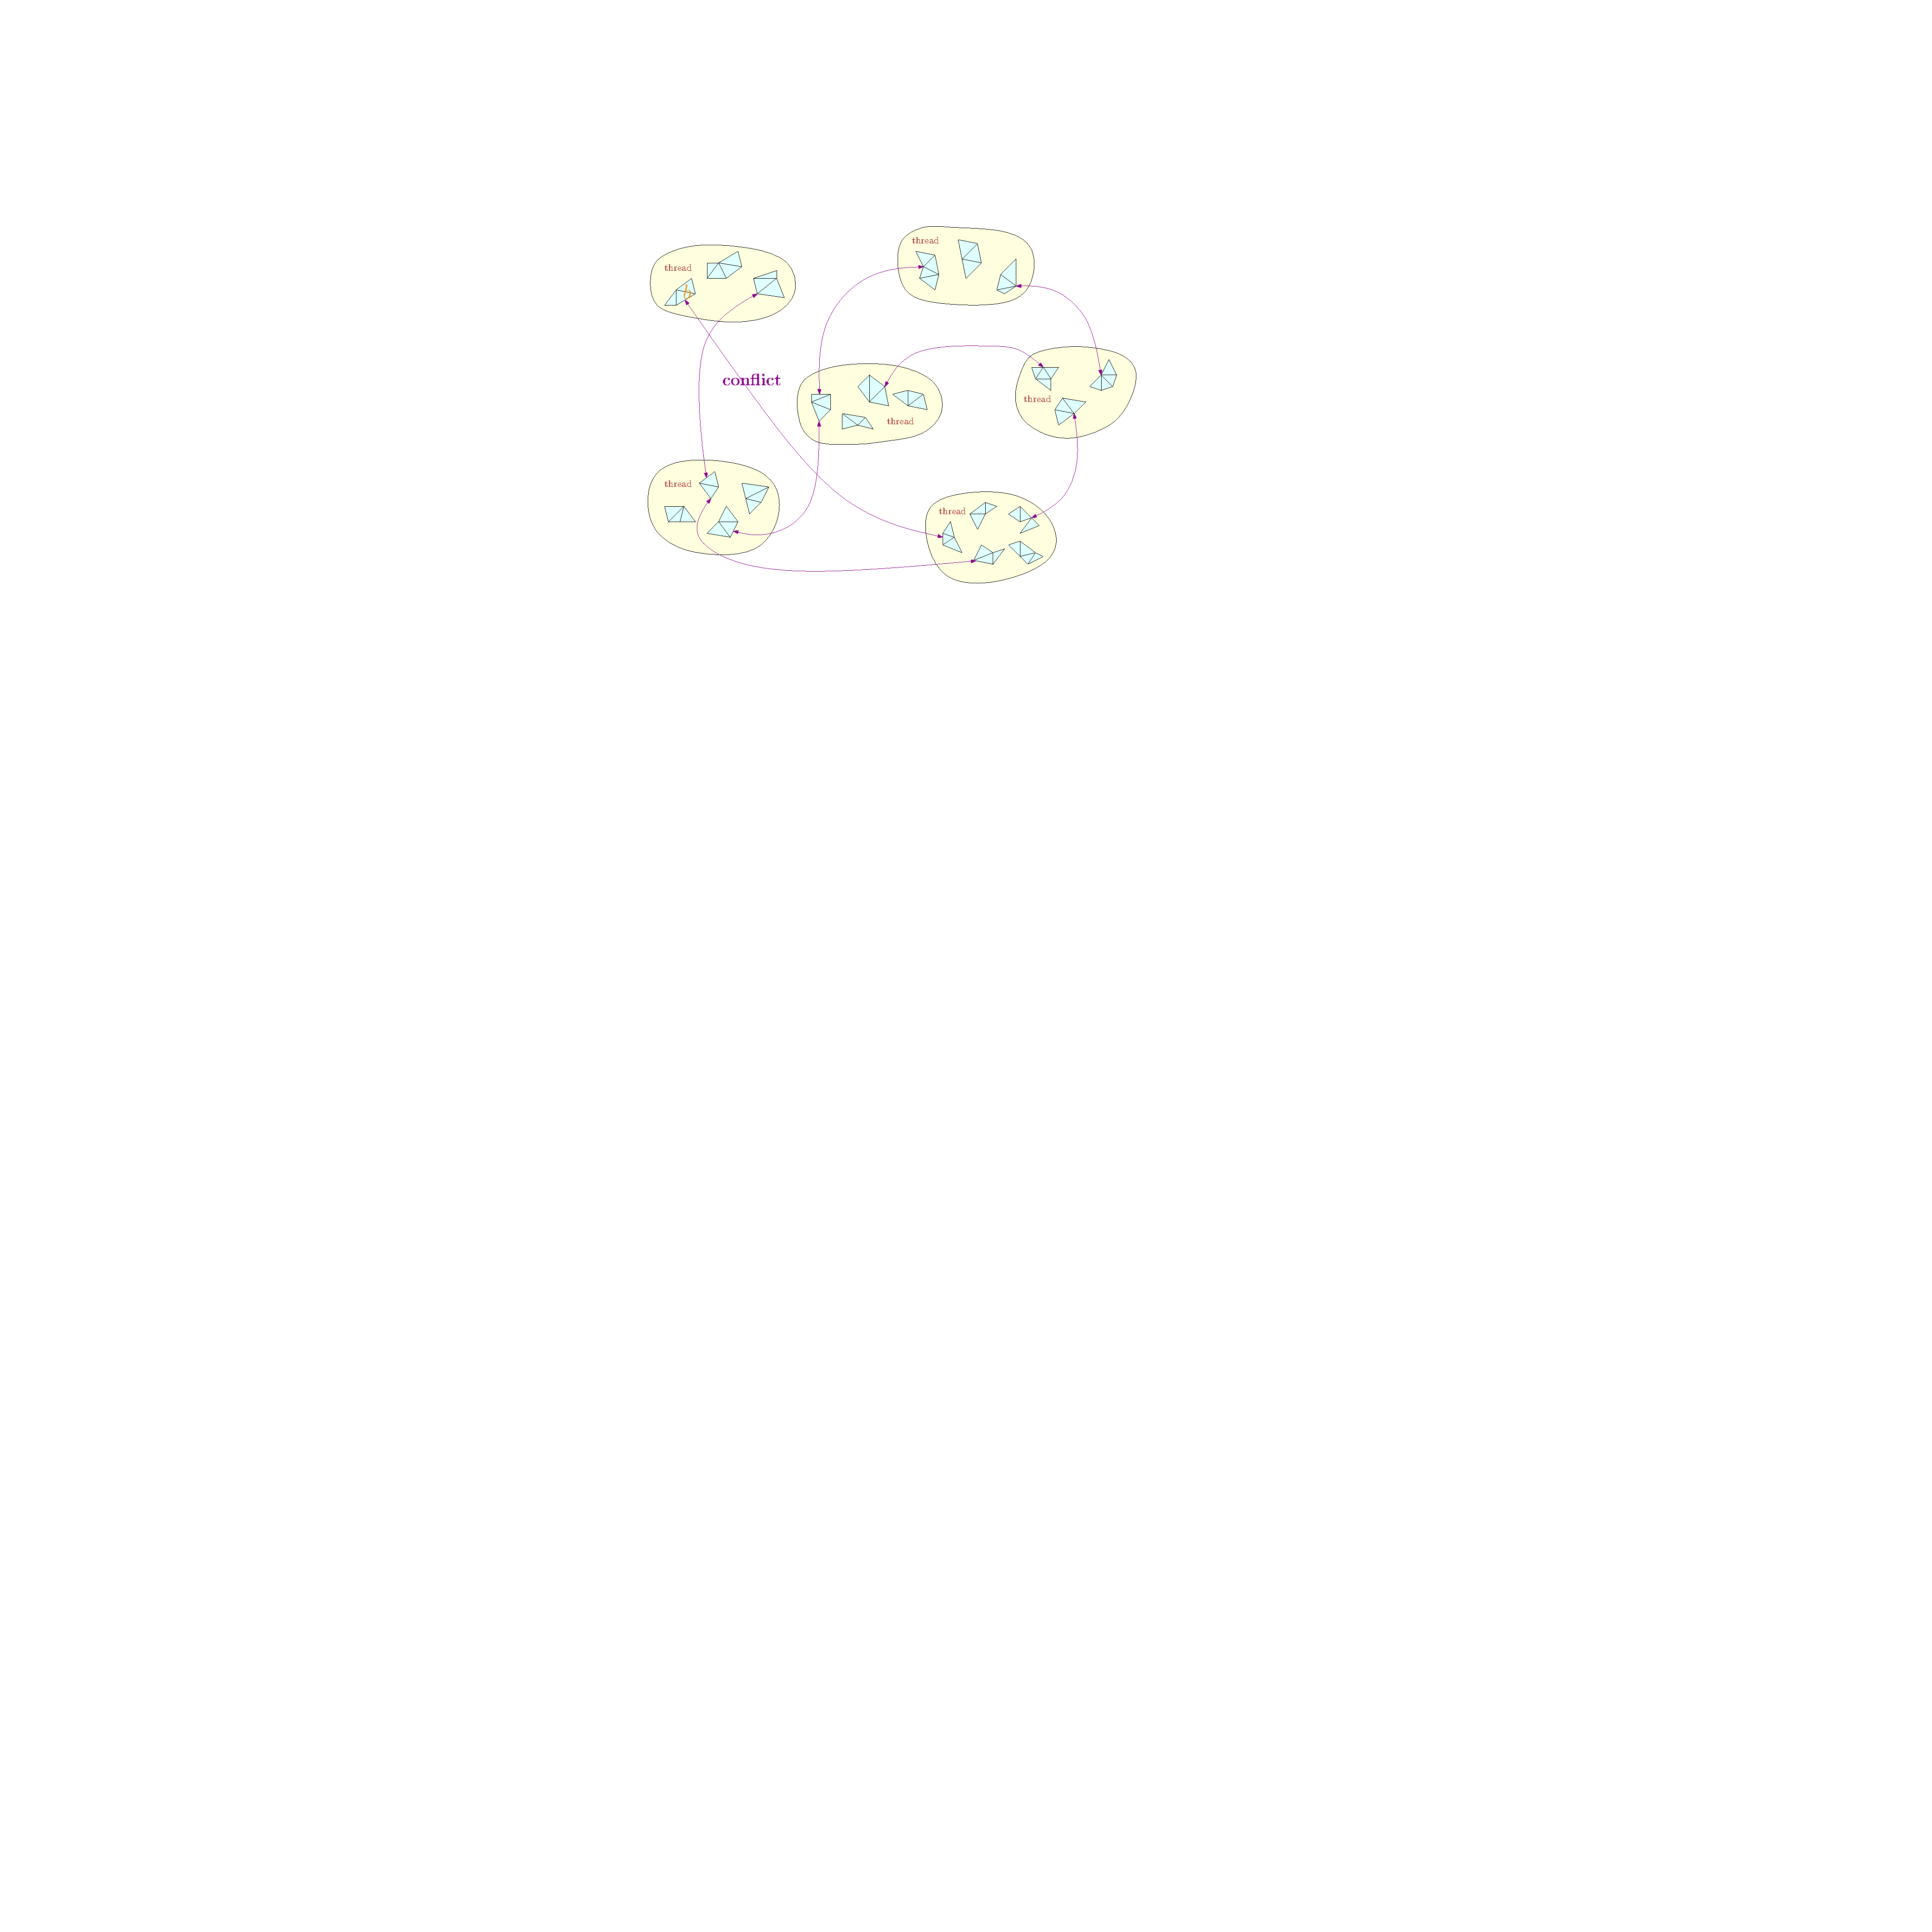
\includegraphics[width=0.6\textwidth]{block-conflicts}
    \caption{Conflicts graph based on block interaction\label{fig:bc}}
  \end{center}
\end{figure}

The current code uses the multi-level partition information to generate
a conflict graph and then schedule the local reduction according to the
conflict graph by using a composite conflict lock.  We call this the
``conflict-based'' approach.  We use the $b$ level partition (see
section \ref{sec:part} for details on multi-level partition and the
meaning of different levels) to overcome the limits on concurrency and
high memory requirements in the previous strategies.  Recall that the
$b$ level partition is a much finer grain partition occurred within each
work thread and that each such partition also preserves the data
locality.  Local reduction is scheduled on each work thread for each of
the $b$ partition a work thread owns.  The execution flow within a
single $b$ partition is the same as it would be executed in sequential.
Different $b$ partitions on different work threads may present race
conditions during the local reduction computation.  However since each
work thread will have many $b$ partition blocks and each block holds its
data locality, the possible chance for a data race is practically small.
For the possible race conditions, we pre-compute a data race map (the
conflict graph) between the possible $b$ blocks on each thread first
during the scheduling phase.  At runtime, each thread checks if a $b$
block to be computed is in conflict with any of the current work
threads.  If not, then the selected $b$ block is committed to be
computed.  If conflict does exist (which should be rare), then the $b$
block is put off and another $b$ block is selected and repeats the
previous process.  Figure \ref{fig:bc} gives an illustration of the
conflicts graph concept based on the $b$ partition.  The arrows in the
graph indicate that the connected $b$ blocks on either end are in
conflict and should not be scheduled at the same time.

There are several steps needed to implement such a scheduling policy and
we discuss the operational overview of each of them.  The first such
task is to build a conflict graph for all the $b$ partitions involved.
This task actually is similar to the graph coloring approach discussed
previously, except that the granularity is much coarser in this case.
If we reuse the previous example and if we partition the input set into
three $b$ blocks: [1,2], [3,4], and [5].  Then according to the original
reduction map: [1$\to$a, 2$\to$b, 3$\to$a, 4$\to$a, 5$\to$b], we can map
each $b$ blocks to a set of output locations: [1,2]$\to$[a,b],
[3,4]$\to$[a], and [5]$\to$[b].  Using a doubly nested loop (with
quadratic complexity), we can establish the conflicts between the three
$b$ blocks: [1,2]$\,\nparallel\,$([3,4],[5]),
[3,4]$\,\nparallel\,$([1,2]), and [5]$\,\nparallel\,$([1,2]).  For
example, [1,2]$\,\nparallel\,$([3,4],[5]) means that the $b$ block [1,2]
can be computed as long as [3,4] and [5] are \emph{not} currently being
computed.  In such a small example, the conflicts are dominating and
this limits the amount of concurrency.  In reality, with large input
size, the conflicts are much more sparse.  Section \ref{sec:perf}
contains a brief discuss of the effectiveness of the current $b$-level
partition in terms of avoiding conflicts.  

\begin{figure}[h]
\begin{lstlisting}[escapechar=@]
// full code in ThreadPartition_simple::generate_conflict_lock in file src/System/thread.cc
void create_conflict_graph(sequence context) {
  // context is the total context for a local reduction rule.
  std::vector<BlockID> blocks_id = partition_by_blocks(context);@\label{code:ln:blockid}@
  std::map<BlockID,entitySet> blocks_target;@\label{code:ln:blocktarget}@
  for(i=0; i<blocks_id.size(); ++i) {
    BlockID b = blocks_id[i];
    blocks_target[b] = vmap_target_exist(blocks[b]);@\label{code:ln:vmapexist}@// computes target entity set for block b
  }
  std::map<BlockID,std::vector<BlockID>> conflict_graph;
  for(t=blocks_target.begin(); t!=blocks_target.end(); ++t) {
    std::vector<BlockID> conflict_blocks;
    entitySet self_target = t->second; // target set of block t
    for(t2=blocks_target.begin(); t2!=blocks_target.end(); ++t2) {
      entitySet other_target = t2->second; // targetset of block t2
      if(self_target & other_target != EMPTY)
        conflict_blocks.push_back(t2.first);
    }
    sort(conflict_blocks.begin(), conflict_blocks.end(), BlockID.cmp());@\label{code:ln:blocksort}@
    conflict_graph[t.first] = conflict_blocks;
  }
}
\end{lstlisting}
\caption{Conflict graph creation\label{fig:cgc}}
\end{figure}

In the current implementation, the conflict graph is built according to
the original reduction maps ([1$\to$a, 2$\to$b, 3$\to$a, 4$\to$a,
5$\to$b] in our example).  This gives the most precise conflicts on all
$b$ blocks with the cost of needing to look into all output locations
(which can be huge and when participating in multiple set operations,
this can be costly).  Figure \ref{fig:cgc} presents a somewhat high
level sketch of the code.  Some of the details have been simplified or
omitted so that the code can be shown in this document.  The type
\lstinline{BlockID} in line \ref{code:ln:blockid} is an abstraction of
the structure used to encode a block's identity on any work thread.  In
practice, it is a two dimensional index with the first index being the
work thread id and the second index being the block id within that
particular work thread.  The \lstinline{partition_by_blocks()} method in
line \ref{code:ln:blockid} breaks a given rule context into different
blocks.  It is defined in the thread partitioner
\lstinline{ThreadPartition} interface presented in section
\ref{sec:part}.  The resulting blocks from the given context are then
stored in a variable (the \lstinline{blocks_id} variable in line
\ref{code:ln:blockid}).  For each of these resulting blocks, we use the
Loci function \lstinline{vmap_target_exist()} to find out the output set
through the maps defined in the local reduction rule.  After this step,
we then use a doubly loop to check if any of these output sets would
intersect with any other ones.  If so, then the two involved blocks
would be in a conflict.  This is a potentially expensive step since the
time complexity is quadratic (proportional to the square of total blocks
involved).  Also note that we sort all blocks in conflict to a
particular block according to a global order on the type
\lstinline{BlockID} (in line \ref{code:ln:blocksort}).  The reason for
this sorting step is ensure the conflict lists for all of the blocks are
in the same order, which is very important for the
\lstinline{ReductionLock} operations described below.

As discussed, the present implementation suffers from a costly time
complexity, particularly when run with a large number of blocks.  Also
such conflict graph is built for each of the local reduction rules
involved in a Loci program.  This could result in a considerable amount
of total scheduling overhead.  There are several ways to reduce this
cost.  In the future, we could have Loci pre-built reduction maps
according to the multi-level partition.  The original reduction map in
the local reduction rule can be regarded as operating on the $p$-level.
If we have a reduction map customized for the $b$-level (e.g., by
coalescing the output locations), then the cost of computing the
conflict graph will be much lower.  In return, we get a less precise
conflict graph.  However in practice, this reduced conflicts precision
may not be an issue due to large number of $b$-level parallelism
available.  Also in a typical Loci program, we could have a large number
of local reduction rules but a small number of local reduction patterns.
For example, several local reduction rules could share the pattern
\texttt{A->B}.  In the present code, each rule will always recompute the
conflict graph.  In the future, if sufficient infrastructure is in
place, we could summarize the local reduction patterns from all of the
local reduction rules.  Then the conflict graph can be built based on
the reduction patterns and be shared among all relevant rules.

Once we have the conflict graph, we will need to build a mechanism to
check if an about-to-be scheduled $b$ block is in conflict with any
currently executing blocks.  We do so by implementing a custom lock (it
is called the \lstinline{ReductionLock} defined in file
\texttt{src/System/thread.h} with implementation in file
\texttt{src/System/thread.cc}).  Each of the $b$ blocks in the system is
assigned a primitive pthread spin lock that supports the
``\texttt{try\_lock}'' query (i.e., returns \lstinline{false} if the
lock is already held by another thread, returns \lstinline{true} and
obtains the lock otherwise).  Before a $b$ block is to be scheduled for
execution, it will need to acquire all the primitive locks correspond to
all other conflicting $b$ blocks.  If any of such acquisition has
failed, then the $b$ block is put back and another one is selected.  The
scheduling finishes when all blocks have been successfully scheduled.  A
very important step in this design is that we agree on a global order on
all of the $b$ blocks and then always acquire the primitive locks
according to such an order (see line \ref{code:ln:blocksort} in Figure
\ref{fig:cgc}).  This is essential to avoid deadlocks.  Figure
\ref{fig:rl} presents a high-level overview of this design.

\begin{figure}[h]
\begin{lstlisting}[escapechar=@]
// in file src/System/thread.h and src/System/thread.cc
class ReductionLock {
  void release(BlockIDIter begin, BlockIDIter end) {
    for(i=begin; i!=end; ++i)
      spin_locks[*i].unlock(); // spin_locks stores a pthread spin lock for every block
  }
  bool acquire(BlockID b) {
    std::vector<BlockID> conflicts = conflict_graph[b];
    for(c=conflicts.begin(); c!=conflicts.end(); ++c)
      if(!c->try_lock())
        release(conflicts.begin(), c);
	return false;
    return true;
  }
  void release(BlockID b) {
    std::vector<BlockID> conflicts = conflict_graph[b];
    release(conflicts.begin(), conflicts.end());
  }
};
\end{lstlisting}
\caption{Reduction lock design\label{fig:rl}}
\end{figure}

With the conflicts graph and the conflicts resolution mechanism, we can
then implement the thread scheduling for local reduction on the $b$
partition level.  The main setup is again the same as other types of
rules discussed previously.  In file \texttt{src/System/thread.h}, the
class \lstinline{ExecuteThreaded_local_reduction} is a
\lstinline{ThreadExecutionModule} and is responsible to schedule and
execute individual blocks.  The class
\lstinline{Threaded_execute_local_reduction} is a
\lstinline{execute_modules} and is responsible to partition the context,
generate the conflict graph, setup the reduction lock, and then generate
and start all needed \lstinline{ExecuteThreaded_local_reduction}.  The
general flow of control is similar to other discussed rule types.  So we
will not show its code.  Figure \ref{fig:etlr} shows the main code for
block scheduling using the previously developed utilities in the class
\lstinline{ExecuteThreaded_local_reduction}.

\begin{figure}[h]
\begin{lstlisting}[escapechar=@]
// in file src/System/thread.h
class ExecuteThreaded_local_reduction: public ThreadedExecutionModule {
  std::list<BlockID> blocks; // total blocks to be scheduled by a work thread
  std::list<BlockID> done_blocks; // records all finished blocks
  ReductionLock& lock; // the reduction lock to be used for a reduction rule
  void execute(fact_db& facts, sched_db& scheds) {
    while(!blocks.empty()) {
      std::list<BlockID>::iterator candidate = blocks.begin();
      while(candidate != blocks.end()) {
	if(lock.acquire(*candidate)) {
	  // successfully acquires the reduction lock for block candidate, schedule it
	  // get an accurate execution context by narrowing it down with the selected block
	  sequence block_seq = thread_control->refine_seq_by_block(*candidate, seq) @\label{code:ln:blocknarrow}@
	  exec_rule->execute_kernel(block_seq);
	  lock->release(*candidate);
	  // put the scheduled block to the finished list
	  std::list<BlockID>::iterator r = candidate;
	  ++candidate;
	  done_blocks.splice(done_blocks.begin(), blocks, r);
	} else // failed to acquire the reduction lock, skip the current block first
	  ++candidate;
      }
      // finally swap the block lists
      blocks.swap(done_blocks);
    }
  }
};
\end{lstlisting}
\caption{Thread scheduling for local reduction\label{fig:etlr}}
\end{figure}

Figure \ref{fig:etlr} presents the main flow of the
\lstinline{execute()} method in the thread work unit class
\lstinline{ExecuteThreaded_local_reduction}.  It maintains two lists of
blocks, one for the blocks to be scheduled and the other for blocks that
have been scheduled.  If a block successfully acquires its reduction
lock, then it is scheduled to be executed on that work thread and then
is put in the finished list.  Otherwise if a block fails to acquire its
reduction lock, it is skipped and another one (if available) is picked.
The entire process ends when the to be scheduled list is empty.  Finally
the method swaps the two lists to prepare for the next run.  Note in
line \ref{code:ln:blocknarrow}, the method
\lstinline{refine_seq_by_block} from the interface
\lstinline{ThreadPartition} is called (see section \ref{sec:part} for
detail).  Its purpose is to get an accurate execution context within the
chosen block.  We could instead pre-compute all such precise contexts
and store them.  However since some of these contexts will likely become
very scattered, the storage requirements for them is likely to be high.
We have therefore chosen to dynamically compute them each time as the
cost of such computation seems to be negligible (according to several
benchmark tests conducted in the past).  As discussed all current Loci
scheduling do not feature dynamic workload balancing support.  A
possible improvement for this code would be to develop a distributed
block migration scheme so that the $b$ block lists on each work thread
can be dynamically balanced at runtime to improve load balance issues.
However developing such an infrastructure is a considerably more complex
task and so far since our $b$ partition also balances the block size and
in our applications the computations on each entity is roughly equal, we
have not had the need to dynamic balance the work load.

\subsubsection{Chomping}
\label{sec:chomp}
The chomping computation can actually be categorized into two types:
there are chomping computations that do not involve any local reduction
computation and those that do.  For chomping without local reduction, a
normal $t$-level scheduling is adequate.  However for chomping with
local reduction, it is necessary to use the $b$-level scheduling
discussed above in the local reduction section.  The scheduling setup is
therefore a bit different.  In file \texttt{src/System/thread.h}, the
class \lstinline{Threaded_execute_chomp} (a subtype of
\lstinline{execute_modules}) is responsible to initialize relevant data
structures and create and start the thread work units.  The overall flow
is similar to any previous rule type scheduling.  The difference is that
we now have two subtypes of \lstinline{ThreadExecutionModule}: the class
\lstinline{ExecuteThreaded_chomp} is used to run chomping graphs that do
not involve local reductions; and the class
\lstinline{ExecuteThreaded_block_chomp} is used to run chomping graphs
that do have local reductions.  \lstinline{ExecuteThreaded_block_chomp}
schedules blocks using a similar programming logic as the class
\lstinline{ExecuteThreaded_local_reduction} discussed in section
\ref{sec:localredux}.  We also define a new type \lstinline{ChompBlock}
to represent a thread partition block whose execution uses the chomping
strategy.  It internally delegates the real computations to a
\lstinline{ExecuteThreaded_chomp}.  Therefore the purpose of the class
\lstinline{ExecuteThreaded_block_chomp} is to coordinate the scheduling
of \lstinline{ChompBlock}.  The purpose of the class
\lstinline{ExecuteThreaded_chomp} is to perform chomping computation for
a given context on work threads.

The size of the chomp is calculated in the class
\lstinline{Threaded_execute_chomp}.  The current implementation still
uses the approach previously used in the sequential version of chomping.
It evaluates the size of a single entity on all involved variables in
the chomping graph and then calculates the chomping size by computing
the ratio of the assumed data cache size and this single entity chomping
variable size.  However this may not be the optimal and in the future,
it may be worthwhile to investigate and test the effects of different
chomping size to determine what works the best.  In the multithreaded
schedule, all work threads need to allocate temporary storage space for
all the chomping variables.  On current architectures, threads do not
usually have their own separate cache.  Caches are usually shared among
several threads (compute cores).  Therefore we probably should reduce
the chomping size accordingly to try to fit the chomping variable
allocation on all work threads into the shared cache.  The
implementation of chomping also deals with several other low level
details.  The source code contains extensive comments that should also
be consulted.

\subsubsection{Recursive computation}
Recursive computation in Loci is the simplest form of computation.  As
discussed, it is not recursive computation that happen at runtime.
Rather the recursion happens at the Loci scheduling phase.  A recursive
computation specification is a particular way of letting the Loci
scheduler to try to deduce all the available entities that can be
applied to a computation.  During the runtime schedule, there is no
explicit recursion happening.  Normally a computation has a straight
computation context and the Loci scheduler is able to construct it in
one pass.  In a recursive rule specification, its computation context is
iteratively computed because the target of the computation might be used
to feedback into the inputs again (which might lead to more entities
being computed).  Thus the Loci scheduler needs to iterate the
scheduling on this computation such that the computation context reaches
a fixed point.  Internally the Loci scheduler generates a list of
schedules for a single recursive computation such that in each step in
the list, there will be no dependency between the inputs and outputs.

For example, a recursive computation may initially output the set [3,4]
from an input set [1,2], however because one of the outputs is also used
as an input, the [3,4] set generated in the first output should be
fed back to the computation again, and this time it generates [5], which
is again a new set.  If we input set [5] to the computation, we will
discover that nothing new is being generated, and then we are done.
Therefore the output should be the set [3,4,5].  However this output
cannot be obtained from a single step since [5] depends on [3,4] being
available.  Therefore Loci generates a list of two individual
computation schedules for this single recursive computation.  The first
one computes [3,4]$\gets$[1,2], and the second schedule computes
[5]$\gets$[1,2,3,4].  Each of the two computation is just another normal
non-recursive Loci computation and therefore can be scheduled for
threads according to the previous strategies discussed.  There are no
specific new types that deals with recursive Loci rules for threads.
Everything is handled as a patch to the method
\lstinline{create_execution_schedule()} in the class
\lstinline{recurse_compiler} in the file
\lstinline{src/System/comp_recurse.cc}.

\subsection{Rule kernel interface}
\label{sec:kernel}
One significant change we have made to the Loci internal is to redesign
the rule infrastructure so that the computation is divided cleanly in
multiple phases.  Previously all rule implementations in the Loci
framework carry a single ``\texttt{compute(seq)}'' method that applies
the computation kernel to all supplied entities in the context
(\lstinline{seq}).  However the \lstinline{compute()} method sometimes
also carries out other non-kernel related tasks (e.g., global variable
change, memory manipulation etc.).  Doing so complicates thread
scheduling because the \lstinline{compute()} method includes both data
parallel and serial tasks.  Figure \ref{fig:old-rule} illustrates such a
design.

\begin{figure}[h]
\begin{lstlisting}[escapechar=@]
// simplified view of the previous Loci rule specification
rule(targets @$\gets$@ source) {
  compute(es) { // "es" is the Loci deduced context for the rule
    targets.resize(); // there may be non-concurrent part present
    for(e : es) kernel(e); // this is the data-parallel kernel call
  }
}
\end{lstlisting}
\caption{Previous Loci rule interface\label{fig:old-rule}}
\end{figure}

In our new rule interface design, the data parallel kernel section is
clearly separated from other potential non-concurrent part.  Figure
\ref{fig:new-rule} presents an overview of the new interfaces.
Essentially this interface distinguishes the computation at entity- and
collection-level.  Computations applied at the entity-level (the kernel)
has transparent data parallelism and can be scheduled independently,
while collection-level computation do not in general have any kinds of
data parallelism.  With this new rule interface, the thread scheduler
can work more effectively.

\begin{figure}[h]
\begin{lstlisting}[escapechar=@]
// simplified view of the new rule interface specification
rule(targets @$\gets$@ source) { // "es" is the Loci deduced context for the rule
  prelude(es) {/* perform any task before applying the kernel */}
  compute(es) { // this is the data parallel kernel call
    for(e : es) kernel(e);}
  postlude(es) {/* perform any task after applying the kernel */}
}
\end{lstlisting}
\caption{New Loci rule interface\label{fig:new-rule}}
\end{figure}

Please refer to Figure \ref{fig:src-overview} to find out the relevant
source code files that contain implementation related to this
functionality (those files marked in the ``threading/non-threading rule
kernel interface'' category).  The associated Loci pre-processor syntax
has also been updated to reflect this newly designed rule interface.
Figure \ref{fig:pp-rule} provides a template of rule computation
specification.  The ``\texttt{prelude()}'' and ``\texttt{postlude()}''
parts in the specification are meant for collection-level computations.
Anything that is intended to be applied to collections should be placed
in these two sections.  The \texttt{prelude()} part is scheduled before
the kernel-level computation and the \texttt{postlude()} part is schedule
after the kernel-level computation.  Example tasks that may go into
these parts may include resizing a container's internal size and I/O
operations etc.  If not explicitly specified, the \texttt{prelude()} and
\texttt{postlude()} sections will default to empty, which means no
operation.  The kernel compute part must be specified in a rule
definition though.  Overall this new interface enables better thread
scheduling decisions.  But it does require the users to become aware of
the difference between entity- and collection-level computations (i.e.,
those computations that can benefit from side-effects free data parallel
scheduling).  Line \ref{code:ln:pre} and \ref{code:ln:post} in Figure
\ref{fig:pw} in Section \ref{sec:pointwise} contain examples of how such
a new rule specification interface is typically used in the thread
scheduler.

\begin{figure}[h]
\begin{lstlisting}[escapechar=@]
// Loci pre-processor definition for a generic rule type
@\$@rule rule_type(...),
  prelude {/* this is the prelude part, defaults to empty */},
  postlude {/* this is the postlude part, defaults to empty */}
  {/* this is the kernel part, must be provided */}
\end{lstlisting}
\caption{New Loci pre-processor rule interface\label{fig:pp-rule}}
\end{figure}

\subsection{Convenience functions}
We have also added the ``\texttt{\$[once]}'' and the
``\texttt{\$[atomic]}'' directives to the Loci pre-processor syntax.
\texttt{\$[once]} supports events that should have a single occurrence
in a parallel environment (but it is not important to specify where in
the parallel and concurrent environment the event occurs).
\texttt{\$[atomic]} groups all operations within its own block and treat
them as a single indivisible operation.

Consider the example presented in Figure \ref{fig:once}.  The rule
specified may be scheduled and executed in any environment, e.g., a
sequential run, a pure MPI-based parallel execution, a pure thread-based
concurrent execution, or a hybrid MPI/thread environment.  Without the
``\texttt{\$[once]}'' directive and its block scope, the output
statement may be executed multiple times in a parallel or concurrent
environment and we will see (possibly garbled) multiple identical output
messages.  With the \texttt{\$[once]} directive, the output message will
only occur once (but we do not care who in the environment actually
executes the output statement).

\begin{figure}[h]
\begin{lstlisting}[escapechar=@]
@\$@rule singleton(...) {
  @\$@[once] {cout<<"execution started\n";}
  // other parts
}
\end{lstlisting}
\caption{\texttt{\$[once]} example\label{fig:once}}
\end{figure}

Internally the ``\texttt{\$[once]}'' directly is implemented as a
condition switch. The global function
\lstinline{is_leading_execution()} defined in file
\texttt{src/System/thread.cc} provides
\lstinline{true}/\lstinline{false} answers to any calling process/thread
whether it is the pre-agreed execution unit for the \texttt{\$[once]}
directive.  The \lstinline{ThreadControl} interface (in file
\texttt{src/System/thread.h}) provides a
\lstinline{is_leading_thread()} interface to determine among all the
threads on an MPI process, which one is the leading thread.  The
function \lstinline{is_leading_execution()} defines a representative
execution path in an execution environment according to the following
rules:

\begin{enumerate}
  \item In a serial execution, the calling execution is the
    representative execution path.
  \item In a multi-process program, the process with MPI rank zero is
    the representative execution path.
  \item In a multithreaded program, the main thread and the first work
    thread are the representative path (in the current design, the main
    and work threads never overlap in execution, so this should not cause
    any problems).
  \item In a hybrid multi-process and multithreaded program, the main
    thread and the first work thread on the MPI rank zero process is the
    representative execution path.
\end{enumerate}

Figure \ref{fig:atomic} presents an example use of the
\texttt{\$[atomic]} directive.  The intention of the operation defined
in the rule is to display the value of a variable to the standard output
stream ``\texttt{cout}.''  If executed in parallel using threads and
without the \texttt{\$[atomic]} directive, then the output may become
garbled since the output code is not atomic.  The atomic directive thus
ensures everything within its block scope is indivisible and as a
result, we will be able to see meaningful output from the computation.
In the file \texttt{src/System/thread.cc}, two functions
\lstinline{global_atomic_region_begin()} and
\lstinline{global_atomic_region_end()} are provided and the
\texttt{\$[atomic]} is translated to enclose its block within these two
functions.  The \lstinline{ThreadControl} interface also provides the
\lstinline{atomic_begin()} and \lstinline{atomic_end()} methods that
ensures atomicity of the code in-between by using a global pthread spin
lock to guard them.  Note that the \texttt{\$[atomic]} directive
currently only works for the multithreaded environment.  It does not
work in a hybrid MPI/thread environment.  

\begin{figure}[h]
\begin{lstlisting}[escapechar=@]
@\$@rule pointwise(var...) {
  @\$@[atomic] {cout<<"variable value = "<<@\$@var;}
  // other parts
}
\end{lstlisting}
\caption{\texttt{\$[atomic]} example\label{fig:atomic}}
\end{figure}

I/O operations are perhaps the most common use of such feature.  However
one should not overuse such atomic regions in the code.  Since the
semantics of a rule's per entity computation (those defined inside the
``\texttt{compute}'' method) is inherently parallel (i.e., can be
scheduled in any order), putting an atomic region inside a rule greatly
limits the performance potential.  Ideally one should not use an atomic
region in a rule and this feature is generally provided for debugging
purpose for a user.  There may be better (but much more complicated)
ways to implement I/O operations in a parallel section.  Since our code
normally does not perform routine I/O operations within a rule, we did
not invest time to optimize the implementation.  Loci already has APIs
in place for special purpose I/O operations.  The
``\texttt{\$[atomic]}'' notation also supports operations other than I/O.

\section{Issues and future improvements}
\label{sec:issues}
Some of the previous sections have mentioned a few issues and possible
updates in the current code implementation.  This section will discuss
some of the important ones in detail.  Maintenance and future
developments of the Loci multithreading system should pay attention to
the discussions presented in this section.

\subsection{Synchronization free local reduction scheduling}
\label{sec:arrow}
So far the biggest possible improvement in the current multithreading
design would be to use a different (and better) strategy to schedule the
local reduction rule on threads.  In the past, we have struggled a lot
on this issue as it is one of the most complicated designs in the
multithreading system and the design had great impact on the performance
not only for the local reduction computations, but also the rest of the
Loci scheduling system.  The initial designs using graph coloring (see
section \ref{sec:localredux}) was not satisfying due to poor performance
and high memory cost.  It was later switched to the multi-level
partition and the conflicts based dynamic scheduling (see section
\ref{sec:part} and \ref{sec:localredux}).  This scheme works
considerably better than the previous designs.  It however has its own
problems.  

\begin{enumerate}

  \item The conflicts based local reduction scheduling still has
    significant thread synchronization embedded at runtime.  This is the
    only place in the current Loci multithreading system where runtime
    work thread coordination is needed\footnote{Technically the global
    reduction rule also involves thread synchronization.  However it is
    a straightforward and isolated step that is much easier to reason
  about and has standard and efficient implementation.}.  Although in
  general the number of conflicts is generally small (see section
  \ref{sec:perf}), it nevertheless exists and is ultimately dependent on
  the Loci program specification.  The existence of such thread
  coordination requirements is the primary reason why the local
  reduction is difficult to schedule efficiently.  

  \item The multi-level partition introduces two levels of partition
    into the multithreading system.  This not only means more processing
    time, it also means that the programming logic is much more
    complicated.  Several special purpose new types had to be designed
    from scratch to deal with the complexity of introducing blocks
    into the system.  

  \item The conflicts graph creation could also become a bottleneck in
    the system.  Section \ref{sec:localredux} mentioned that currently a
    quadratic time algorithm is used to create the graph and each local
    reduction rule recreates the conflict graph even though some of the
    reduction patterns can be the same between several rules.  Improving
    these current issues is possible, but may not be simple and
    straightforward.

\end{enumerate}

\subsubsection{Arrow view and arrow partition}
We have indeed developed a new proposal to schedule local reduction
computation on multiple concurrent threads that is completely
synchronization free and logically easier to reason about.  We think
that this proposal is feasible and actually if designed and implemented
appropriately, will also expand the Loci framework's capability
considerably.  However due to the current Loci architecture design and
implementation, this new proposal requires significant rework of the
Loci architecture to realize.  We will outline the main ideas first and
then discuss several ways to approach the implementation and their
challenges.

\begin{figure}[h]
  \begin{center}
    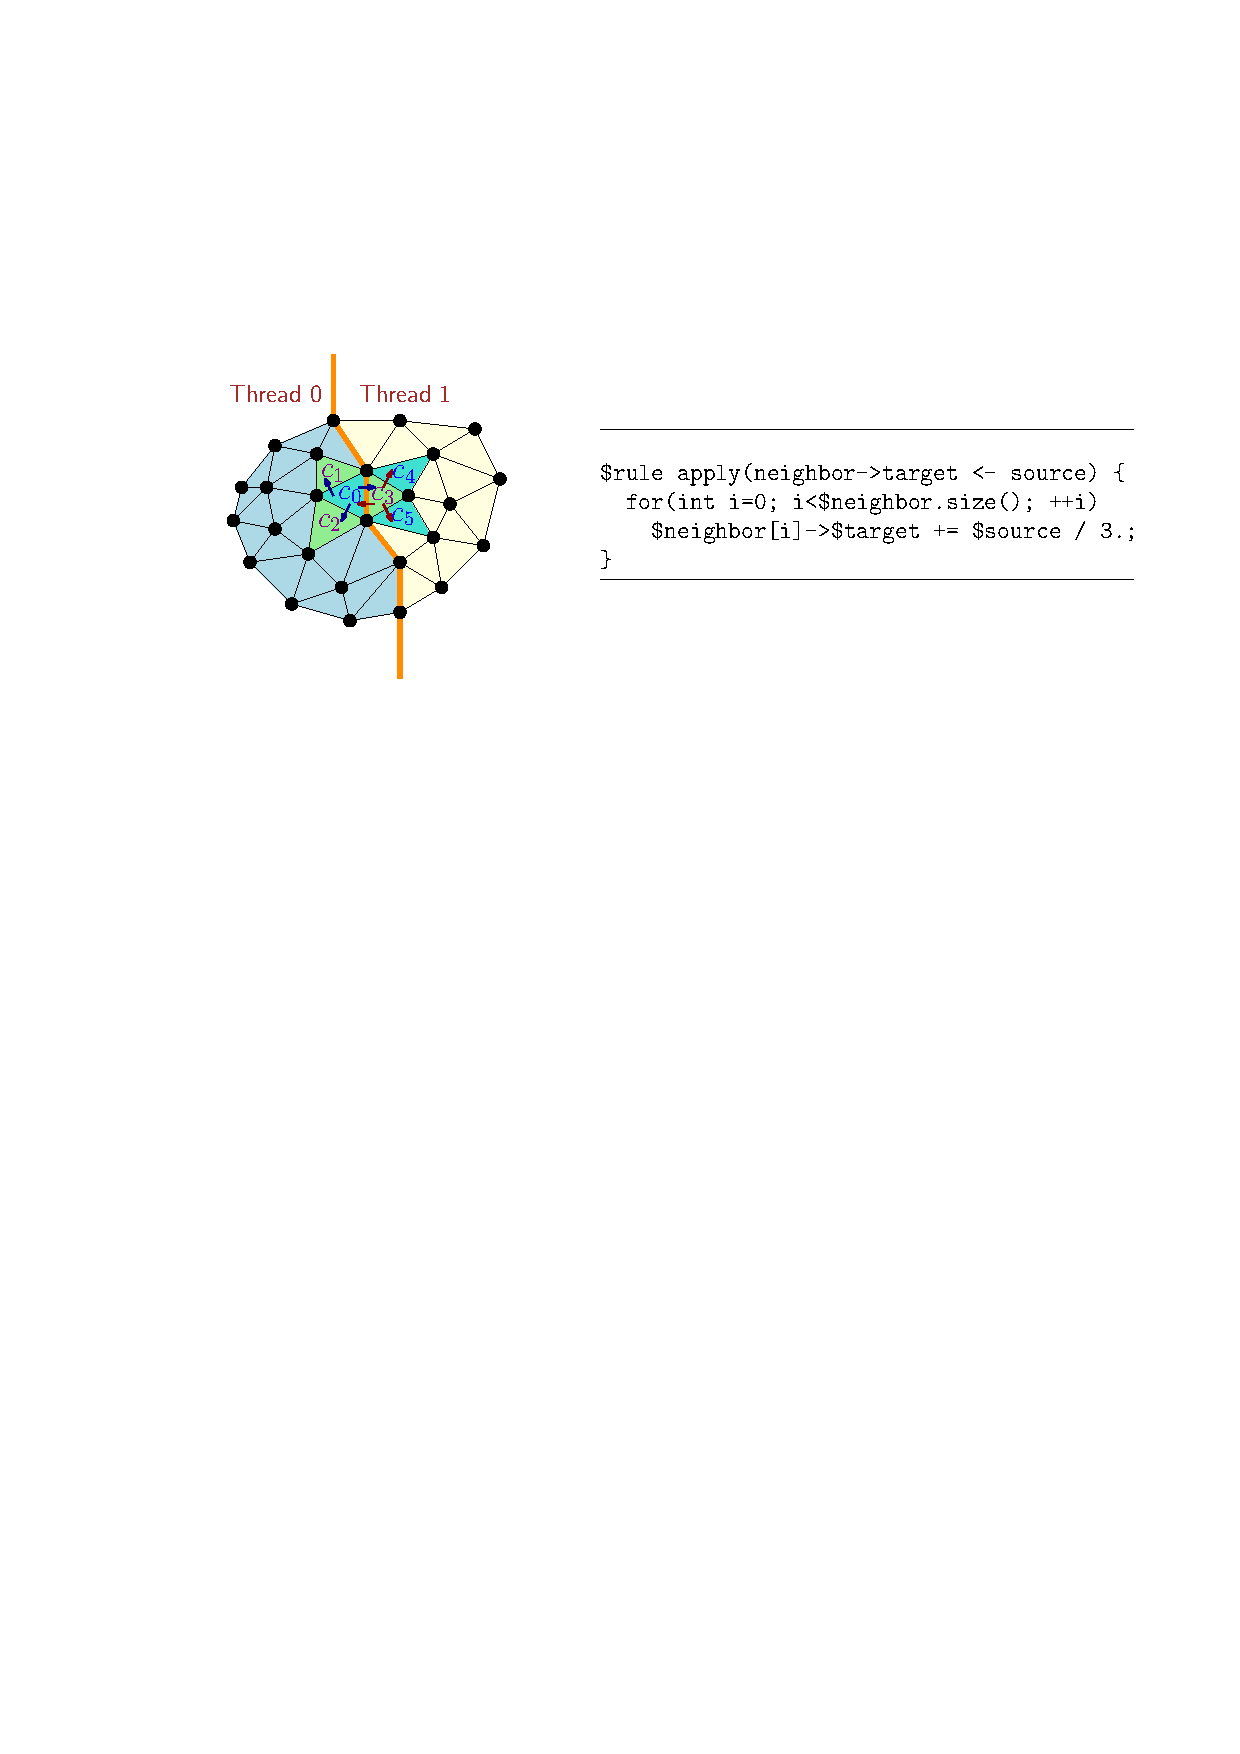
\includegraphics[width=0.75\textwidth]{arrows}
    \caption{Arrow view of local reduction\label{fig:arrows}}
  \end{center}
\end{figure}

Figure \ref{fig:arrows} shows an example of a Loci local reduction rule
(on the right side) and visualization of the computation on a small 2D
mesh (on the left).  The local reduction sums a value on each cell in
the mesh to all of its neighboring cells.  The small arrows in the
figure represent the direction of data flow (the accumulation of values)
from the source of the local reduction to the target of the local
reduction.  The thread that ``owns'' an arrow will need to read data
from the site at the arrow's source and write data to the site at the
arrow's destination.  Whenever an arrow on a thread points to a site
inside another thread's partition, then a potential synchronization
problem arises.  The reason why a particular local reduction scheduling
scheme cannot avoid thread synchronization is because it cannot arrange
all arrows on any thread to \emph{not} pointing outside its own
partition.  This is true for all the schemes discussed so far
(replication, graph coloring, and dynamic conflicts resolution).  In
fact, all other current numerical software we are aware of have this
problem.  The root cause that a particular scheme cannot contain arrow
direction to be within a thread is because we always group arrows based
on their origination.  In the example shown in Figure \ref{fig:arrows},
all previous scheduling policies group the three arrows pointing outward
of cell $c_0$ together on thread zero, so is the case for cell $c_3$ on
thread one.  Under such a partition, thread synchronization is
unavoidable.  We have not seen any discussion of synchronization free
local reduction multithread scheduling in the current literature.

However if the Loci framework could support these arrows as a
fundamental computational and scheduling unit, then multithreaded local
reduction can be easily scheduled synchronization free.  We will just
need to partition all of the arrows among the threads such that no arrow
on any thread will be pointing outside of its partition.  It is okay
to have an arrow on a thread to come from another thread partition, i.e.,
the arrow's origination can be from another thread partition.  This just
amounts to read data from another thread partition, which is safe to
do\footnote{So long as the arrows do not represent in-place update.
However local reduction computation with in-place update is inherently
non-deterministic, even in the sequential case.  E.g., consider the Game
of Life implementation.}.

An arrow is equivalent to a single entry in a Loci map in the Loci
framework.  For example, if we have a Loci map $m$ where $m[c_0] = c_1$,
$m[c_0] = c_2$, and $m[c_0] = c3$, etc (this would be a
\lstinline{multiMap} in the Loci container type).  Then each of these
entry amounts to an arrow.  Present Loci framework uses entity (i.e.,
$c_0$, $c_1$, and $c_2$ etc.) as the fundamental unit.  Thus we can only
compose and schedule computation on entities.  For example, using the
previous example, when we schedule computations related to map $m$, we
can only supply entities like $c_0$, $c_1$, and $c_3$.  When an entity
such as $c_0$ is feed to a map (in this case a \lstinline{multiMap}),
then we will automatically get the image as a set of $[c_1,c_2,c_3]$,
i.e., we will be forced to group the three arrows pointing outward of
$c_0$ together.  This is the reason why we cannot define and compose
arrows in the Loci framework.

It is perhaps very powerful to make arrow the fundamental unit in
composition and scheduling in the Loci framework instead of the
entities (entities are merely abstraction for data locations).  Arrows
are an even fine grain and low level abstraction in computation compared
to the entities.  It provides an abstraction that is more elegant and
composable.  Under the arrow abstraction, maps are just collections of
arrows.  Computation which do not involve maps can be viewed as going
through an identity map, which makes scheduling based on arrows
universal (this is a special case, in which an arrow degenerates to be
equivalent to an entity).

\subsubsection{Ad hoc emulation of arrow partition}
Properly implementing the arrow abstraction and its scheduling in the
Loci framework is not an easy task.  It is also a new concept and we
perhaps do not have a full grasp of all its implications.  Incorporating
arrows in the Loci framework would certainly have a wide range of
effects and applications.  However if we only want to make scheduling
multithreaded local reduction synchronization free, there is an ad hoc
way of emulating arrows and its partition among threads.

In the left part of Figure \ref{fig:arrows}, we illustrated a normal
partition in Loci.  Under such a partition, any cell in the mesh (an
entity) is owned by a unique thread.  For example, the cells
$[c_0,c_1,c_2]$ are owned by thread zero and the cells $[c_3,c_4,c_5]$
are owned by thread one.  The arrows are captured in a single map.
Suppose we call such a map $m$.  The part of $m$ accessible on thread
zero is called $m_{t_0}$ and the part of $m$ accessible on thread one is
called $m_{t_1}$.  Then thread zero will make use of the mapping
$m_{t_0}[c_0] = c_1$, $m_{t_0}[c_0] = c_1$, $m_{t_0}[c_0] = c_2$ in its
local reduction.  And thread one will make use of the mapping
$m_{t_1}[c_3] = c_0$, $m_{t_1}[c_3] = c_4$, and $m_{t_1}[c_3] = c_5$ in
its local reduction computation.  Since each thread has a single map and
can only retrieve the entire image set of a single entity input, the
schedule will have synchronization problems.

If instead we split the map $m$ on each thread into two copies and
spread it contents into these two copies, then we could emulate an arrow
partition.  For example, still using the previous example, we split
$m_{t_0}$ into $m^o_{t_0}$ and $m^*_{t_0}$ on thread zero, where
$m^o_{t_0}[c_0] = c_1$, $m^o_{t_0}[c_0] = c_2$, and $m^*_{t_0}[c_3] =
c_0$.  And we also split $m_{t_1}$ into $m^o_{t_1}$ and $m^*_{t_1}$ on
thread one, where $m^o_{t_1}[c_3] = c_4$, $m^o_{t_1}[c_3] = c_5$, and
$m^*_{t_1}[c_0] = c_3$.  We can see that $m^o_{t_0} \cup m^o_{t_1} \cup
m^*_{t_0} \cup m^*_{t_1} = m_{t_0} \cup m_{t_1} = m$.  This effectively
forms a partition of arrows by using multiple maps.  Now when thread
zero runs the local reduction through $m^o_{t_0}$ and $m^*_{t_0}$, and
thread one runs the local reduction through $m^o_{t_1}$ and $m^*_{t_1}$
concurrently, there will be no interference and no synchronization will
be needed.  In practice we will merge $m^o_{t_0}$ and $m^*_{t_0}$ into a
single map $m^b_{t_0}$ and similarly we merge $m^o_{t_1}$ and $m^*_{t_1}$
into $m^b_{t_1}$.  Thus the map $m^b_{t_0} \cup m^b_{t_1}$ is equivalent
to the original map $m$, and $m^b_{t_0}$ and $m^b_{t_1}$ form an reorder
of the maps $m_{t_0}$ and $m_{t_1}$.  In this way, if the local
reduction rule use the new maps $m^b_{t_0}$ and $m^b_{t_1}$ instead of
the original maps $m_{t_0}$ and $m_{t_1}$ on corresponding threads, then
we obtain a synchronization free multithreaded local reduction schedule.
We can use map reordering on threads to emulate the effects of arrow
partition.

Implementing such a scheme is however complicated as well in the present
Loci framework.  The complication comes from the limitation in the Loci
framework to swap individual variable representation in a rule kernel.
The current Loci rule \lstinline{execute_modules} will need to use the
interface \lstinline{initialize()} in type \lstinline{rule_impl} to
setup a connection between the variables declared in a rule and storage
spaces in the Loci \lstinline{fact_db}.  This step makes replacing a
single (or a few) individual variable storages (perhaps generated
locally and not in the \lstinline{fact_db}) difficult.  This is perhaps
still doable with moderate refactoring of the current interface.
However the Loci framework is unable to change the source code specified
in a rule kernel as well, which makes replacing the original map with an
enhanced reordered map impossible.  Consider the example given in Figure
\ref{fig:genredux}.  This reduction happens through a chain of maps and
the source code in C++ encodes the reference of all the maps involved in
the chain.  When we generate a reordered map, we do not want to reorder
all of the individual maps in chain.  Instead we wanted to replace the
chain \texttt{\$m0->\$m1->\$m2} with a single reordered map, i.e., we
would want to flatten the chain first and then reorder the flattened map.
But we cannot change the C++ source code in the kernel to match up.  The
only feasible way in the current setup seems to have an intelligent Loci
pre-processor that can generate new C++ source code.

\begin{figure}[h]
\noindent\rule{0.85\textwidth}{0.4pt}
\begin{verbatim}
  $rule apply(m0->m1->m2->target <- source) {
    $m0->$m1->$m2->$target += $source / 3.;
  }
  // ...... corresponding C++ source code for the kernel
  void calculate(Entity e) {
    target[m2[m1[m0[e]]]] += source[e] / 3.;
  }
\end{verbatim}
\noindent\rule{0.85\textwidth}{0.4pt}
\caption{A general Loci reduction rule\label{fig:genredux}}
\end{figure}

%%\begin{figure}[h]
%%  \begin{center}
%%    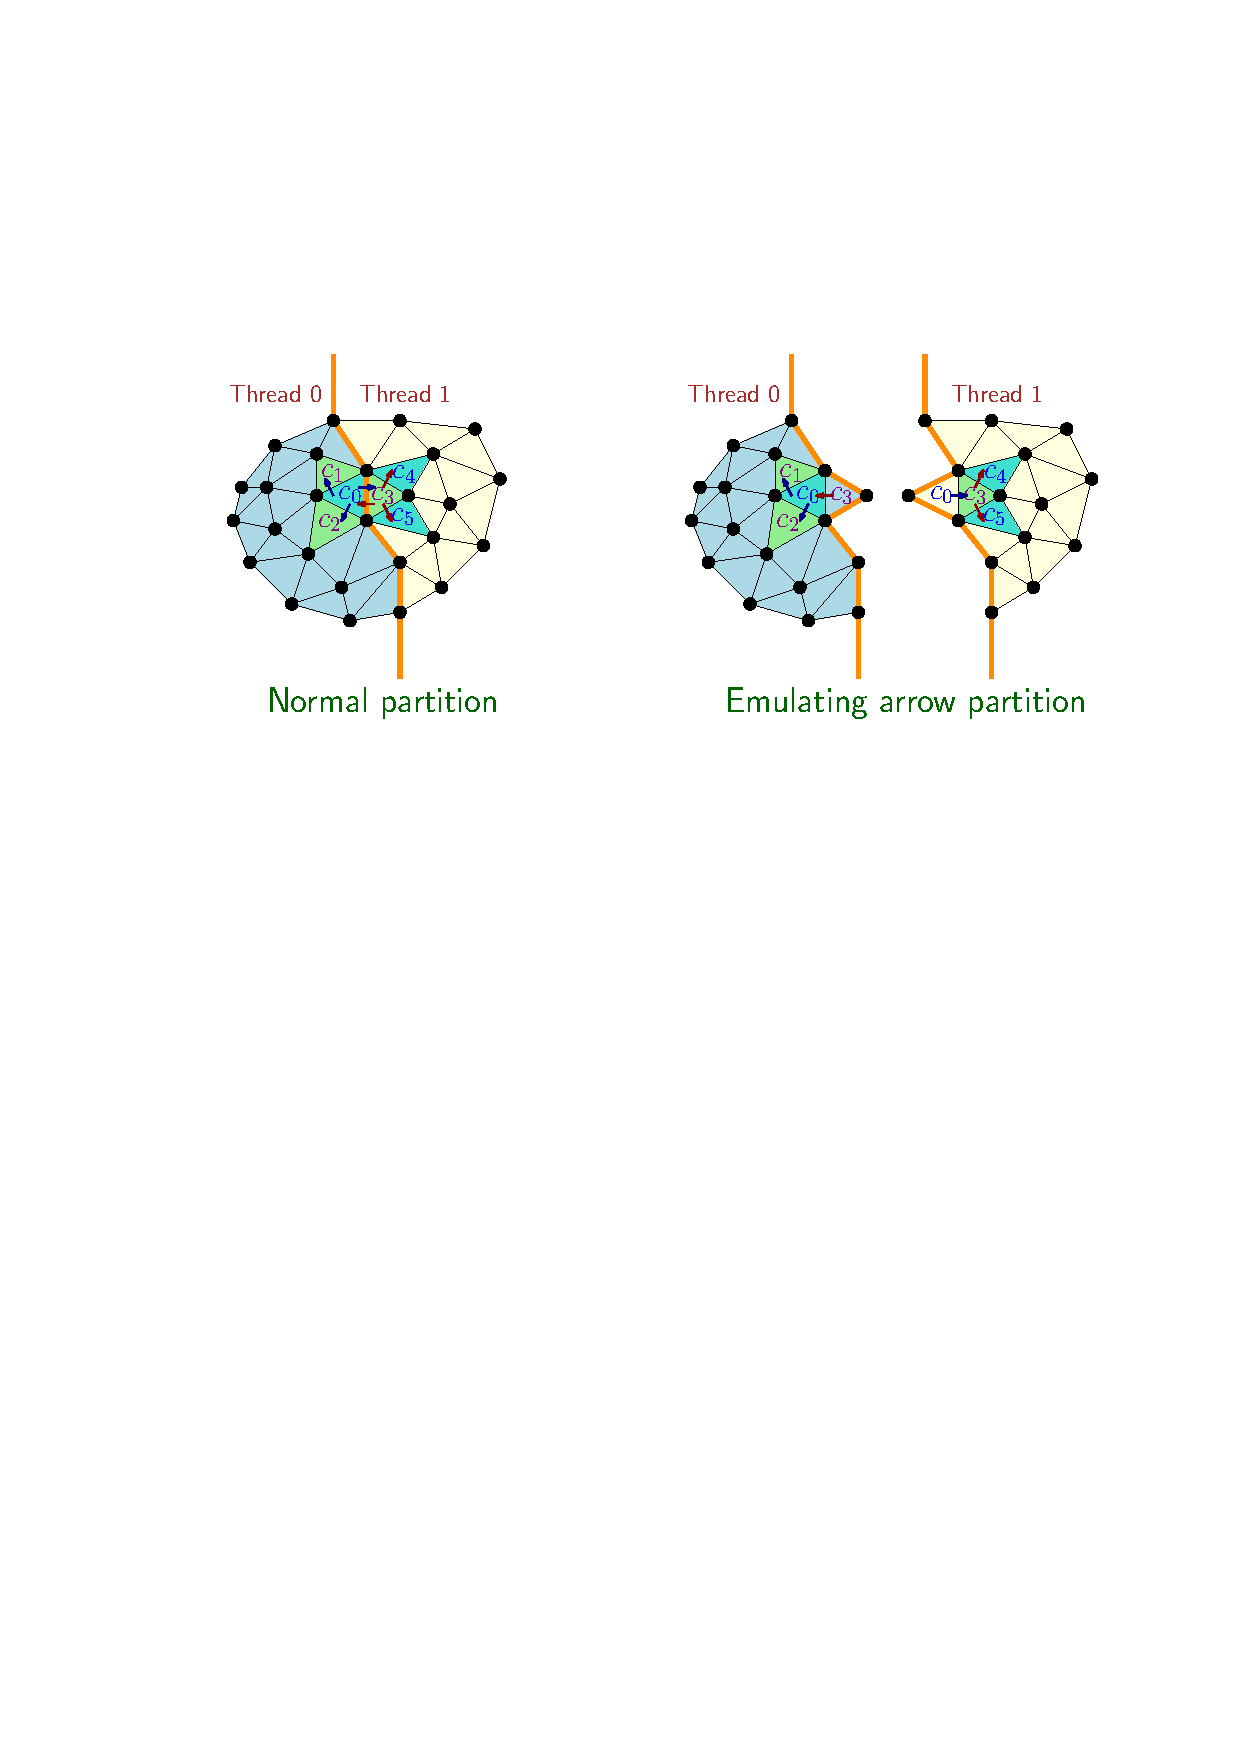
\includegraphics[width=0.75\textwidth]{arrow-emulate}
%%    \caption{Emulating arrow partition\label{fig:eap}}
%%  \end{center}
%%\end{figure}

\subsection{Hidden synchronization}
\label{sec:hiddensync}
The current Loci framework uses a subscriber pattern in the storage
hierarchy design.  A storage allocation (\lstinline{storeRep}) can be
shared among different names (called the shell, e.g., a
\lstinline{store}) and the shells also maintain pointers to the
underlying storage memory location for direct access.  Whenever a
storage allocation changes itself, it calls the interface
\lstinline{dispatch_notify()} to update the shell pointers (which
defines the routine \lstinline{notification()} as a callback).  This
mechanism is necessary to use a list to record who to send the
notification in case it is needed.  In a multithreading environment,
such a subscriber list is shared among all the threads and will need to
be guarded by a thread lock to prevent data corruption.  This then
creates a hidden thread synchronization cost.  Since the Loci storage
interface is ubiquitous in the system, this can be a concern for thread
performance.

A general solution to this problem might be to use more effective atomic
variables instead of mutual exclusion locks to guard the subscriber list
(such as those atomic constructs supported in the c++11 standard).  A
better way is to redesign the storage hierarchy in Loci altogether to
remove such hidden thread synchronization cost completely.  Currently we
have designed some special interfaces in the storage hierarchy to help
mitigate this problem.  A special copying routine
\lstinline{fast_copy()} has been added to the \lstinline{storeRep} type.
Currently only the \lstinline{paramRepI} class implements this new
interface.  Other \lstinline{storeRep} types delegate the implementation
to the normal \lstinline{copy()} routine.  Some of the
\lstinline{storeRep} types, notably the \lstinline{paramRepI}, will need
to invoke the \lstinline{dispatch_notify()} interface, which will cause
thread locks to be acquired and released.  While it may be the case that
in the multithreading execution, there is only one or no subscriber in
the list and only one thread will be accessing the list, having to
acquire and release the locks may still cost a little performance.
Instead the \lstinline{fast_copy()} routine implemented in the
\lstinline{paramRepI} class skips the \lstinline{dispatch_notify()}
call.  But it is then only safe to call the \lstinline{fast_copy()} on a
\lstinline{paramRepI} only if it is not linked to any of the shell
containers.  This is the case in global reduction scheduling and so it
is used (see line \ref{code:ln:fastcopy} in Figure \ref{fig:gr} in
section \ref{sec:gr}).

There are several other issues related to this general problem in the
Loci framework that a developer needs to be aware of in a multithreading
environment.  The current implementation of the \lstinline{entitySet}
type uses a similar setup.  It uses a ``handle'' type to share data via
a counted pointer.  This reference counted pointer is not protected for
thread access though.  And this will cause certain calls involve
\lstinline{entitySet} to fail in a multithreaded environment.  An
example would be that calling the \lstinline{domain()} function on a
shared container will likely to fail since the \lstinline{entitySet}
that represents the domain being returned by the call will be copied,
which is not thread safe\footnote{This is a hard lesson learned from a
  seemingly innocent bug in the code, which took some time to understand
and fix.}.  Another potential error would be to perform
conversion between the \lstinline{sequence} and the
\lstinline{entitySet} types.  Currently converting to an
\lstinline{entitySet} from a \lstinline{sequence} is thread safe,
however, converting to a \lstinline{sequence} type from an
\lstinline{entitySet} type is \emph{not} thread safe due to the way the
internal data sharing is implemented.  Note however that we do not want
to protect the underlying shared data in \lstinline{entitySet} since
doing so will possibly severely degrade thread performance because
\lstinline{entitySet} is the most important foundation in the current
Loci implementation.

\subsection{Thorny Loci abstractions and semantics}
\label{sec:thornyabs}
Currently some of the Loci abstractions and semantics are also causing
inconvenience in several situations.  These are probably manifestations
of the design problems in the associated Loci abstractions and
semantics.  Future developments would need to consider improving or
redesigning these and possibly other related abstractions and semantics.

The first inconvenience comes from the need to frequently convert
between the \lstinline{sequence} and \lstinline{entitySet} types in the
scheduler and during runtime execution of certain rule kernels.  These
two types are closely related (they share a large portion of underlying
implementation), yet they are not entirely compatible (e.g., the ``-''
operator is only defined on \lstinline{entitySet} and not on
\lstinline{sequence}).  The current \lstinline{compute()} interface in a
\lstinline{rule_impl} type takes a \lstinline{sequence} to represent the
execution context.  While many operations on variables produce
\lstinline{entitySet} type as a result (such as the
\lstinline{domain()}, \lstinline{image()}, and many set operations).
The multithreading code does a lot of set manipulations and
calculations.  In many cases, we are forced to convert between the
\lstinline{sequence} and the \lstinline{entitySet} types just so we can
call the functions needed (e.g., converting an \lstinline{entitySet} to
a \lstinline{sequence} so that we can use it as the context for a rule
to compute).  Doing these conversions (especially frequently) is not
only costly (particularly when the \lstinline{entitySet} contains a
large number of segments), but it may also be thread unsafe (such as
when converting from an \lstinline{entitySet} to a
\lstinline{sequence}).  In fact, if we change the rule context type to
be \lstinline{entitySet} instead of the current \lstinline{sequence}
type, then most of these conversion problems will go away.  It is also
more appropriate to use the \lstinline{entitySet} type as the general
rule context type since a fundamental Loci rule semantics is referential
transparency in a rule kernel.  The rule kernel can be applied to any
entity in its context regardless of order.  Then it makes sense to use
\lstinline{entitySet} as the context type since it is just a collection
of entities without order.  While the purpose of \lstinline{sequence} is
to encode a total order of the entities collected.  In the
multithreading schedule, such transparent execution of the rule kernel
is also the foundation of the data parallelism employed.  Therefore we
strongly suggest the rule context type be changed to
\lstinline{entitySet} from \lstinline{sequence} in future revisions of
the Loci framework.  Doing so will likely produce more efficient code
and enforce the Loci semantics assumptions.

In practice a Loci rule can have side-effects and there is no way to
enforce side-effect free rule specifications in the Loci abstraction.
Then to ensure the correctness of a schedule, certain procedures must
always be (re)evaluated.  An example comes from the implementation of
chomping.  When we run the chomping schedule, we will need to allocate
small storage spaces for all those chomping variables.  Ideally since
these storage spaces are quite small (after all, they should fit inside
a small cache), we could create them once and keep them for repeated
reuse.  However there is no guarantee that the variables involved in
chomping would be the same type.  It is possible that a rule can set
different variable types during different invocation (e.g., by
changing the vector size of a \lstinline{storeVec}), thus invalidating
the previously created chomping storage.  Therefore to ensure complete
correctness, every time before the chomping schedule runs, we have to
query the \lstinline{fact_db} for all chomping variables and recreate
the temporary chomping storage again.  In reality probably no current
Loci rules will change a variable type in different execution time
(indeed this is the assumption made in the older sequential chomping
code so it only query the \lstinline{fact_db} once).  However there is
no guarantee that this will not happen.

Another potential problem related to side-effects and execution orders
also exists in the chomping schedule.  As section \ref{sec:kernel}
discussed, a rule now has three execution points, the
\lstinline{prelude()} and \lstinline{postlude()} are now used to specify
non-data parallel computations, and \lstinline{compute()} is used to
specify data parallel entity-level computations.  A normal schedule
of a rule would call \lstinline{prelude()} first, followed by
\lstinline{compute()}, and then finally the \lstinline{postlude()}
interface.  If a group of rules (e.g., \lstinline{r0} and
\lstinline{r1}) is not run in chomping mode, then the order of their
execution will be: \lstinline{r0.prelude()},
\lstinline{r0.compute()}, \lstinline{r0.postlude()},
\lstinline{r1.prelude()}, \lstinline{r1.compute()},
\lstinline{r1.postlude()}.  However if the rule group is run in chomping
mode, then they will effectively become a single execution unit, i.e.,
the chomping execution of \lstinline{r0} and \lstinline{r1} has to occur
together.  But the \lstinline{prelude()} and \lstinline{postlude()}
cannot be chomped and have to be called outside of the chomping.  The
current setup uses this order: \lstinline{r0.prelude()},
\lstinline{r1.prelude()}, \lstinline{chomping(r0,r1)},
\lstinline{r0.postlude()}, \lstinline{r1.postlude()}.  This is a
different order than the non-chomping run and if there are side-effects
in any of these interface specifications, then the chomping and
non-chomping execution results may be different.  This is usually not a
problem (and has not been a problem so far for all Loci applications).
But again there is no guarantee offered by the Loci framework.

We can instead leave these semantics issues there and rely on the fact
that probably no Loci rule specifications will break the current
assumptions made in the code.  However these do cause some unease and
discomfort.  Worse, they may be forgotten in the long run and if future
application specifications do violate some of these assumptions, then
weird bugs may appear and will be hard to understand, particularly if
multiple of such assumptions are embedded in the Loci implementation and
interact in some unpredictable and complex ways.  Having clean, strict,
and well behaved semantics is thus important.

\section{Preliminary tests and assessments}
\label{sec:perf}
For completeness purpose, we include a preliminary performance
assessment of the multithreading system in this section.  This is only a
preliminary assessment based on a 2016 version of Loci.  So it is just
for reference only.  The brief performance evaluation is carried on a
simple ``\texttt{euler}'' program constructed using the Loci framework
with various threading options enabled.  Several moderately sized input
grids are used.  Experiments using eight processes/threads and less are
conducted on a desktop workstation with 3.7GHz Intel Xeon E5-1630 CPU
(four physical cores with eight hardware threads) and 32GB of memory.
Experiments utilizing beyond eight processes/threads are performed on a
Linux cluster whose single node consists of 2.8GHz Intel Xeon E5-2680 v2
CPU (ten physical cores with 20 hardware threads) and 64GB of memory.

The \texttt{euler} program is run in chomping and non-chomping modes.
Table \ref{tab:euler-mode-stat} shows the total and threaded computation
of each rule type.  It may seem strange why not all of the pointwise
computations are threaded.  This is mainly because some of the
pointwise computations are inherently sequential (such as I/O
processing) and some may contain non-safe operations for threads.

\begin{table}[h]
  \begin{center}
    \begin{threeparttable}
      \caption{Type of computations in the \texttt{euler} program\label{tab:euler-mode-stat}}
      \begin{tabular}{|l|c|c|c|c|c|}
	\hline
	& pointwise & global reduction & local reduction & chomping &
	recursion\\
	\hline
	with chomping & 25/37\tnote{1} & 1/1 & 2/2 & 3/3 & 0/0\\
	no chomping & 38/50 & 2/2 & 6/6 & 0/0 & 0/0\\
	\hline
      \end{tabular}
      \begin{tablenotes}
      \item [1] This denotes 25 computations are threaded out of a total
	37.  The same goes for the rest of the table.
      \end{tablenotes}
    \end{threeparttable}
  \end{center}
\end{table}

Table \ref{tab:euler-wall-small} presents the wall timing results of the
\texttt{euler} program execution with different parallel options.  The
execution is carried using a single process with eight working threads,
two MPI processes each with four working threads, four MPI processes
each with two working threads, and purely eight MPI processes.  The
two middle configurations represent a hybrid parallel execution and is
the main intended use of the threading infrastructure (together with MPI
parallelism).  All measurements are in seconds.  The execution timing is
the total time taken to execute 100 iterations and does not include any
Loci pre-processing time.  In these measurements, each working thread
uses a 25-block division. The numbers in the parentheses represent the
slow down when compared to the eight MPI-process run (which represents
the highest performance so far).
\begin{table}[h]
  \begin{center}
    \caption{Wall time of \texttt{euler} execution (small grid, 25 blocks per thread)\label{tab:euler-wall-small}}
    \begin{tabular}{|l|c|c|c|c|}
      \hline
      & 8 threads & 2 mpi 4 threads & 4 mpi 2 threads & 8 mpi\\
      \hline
      with chomping & 114.2 (18.1\%) & 101.1 (4.6\%) & 99.4 (2.8\%) & 96.7\\ 
      no chomping & 145.2 (26.3\%) & 122.7 (6.7\%) & 119.5 (3.9\%) & 115.0\\
      \hline
    \end{tabular}
  \end{center}
\end{table}

\begin{table}[h]
  \begin{center}
    \caption{Wall time of \texttt{euler} execution (large grid, 25 blocks per thread)\label{tab:euler-wall-large}}
    \begin{tabular}{|l|c|c|c|c|}
      \hline
      & 8 threads & 2 mpi 4 threads & 4 mpi 2 threads & 8 mpi\\
      \hline
      with chomping & 447.1 (11.1\%) & 408.0 (1.3\%) & 405.1 (0.6\%) &
      402.6\\ 
      no chomping & 564.3 (17.1\%) & 490.1 (1.7\%) & 495.1 (2.7\%) &
      482.1\\
      \hline
    \end{tabular}
  \end{center}
\end{table}

Table \ref{tab:euler-wall-large} shows the timing results of the same
configuration as measured in Table \ref{tab:euler-wall-small}, except
that the program is run on a larger input grid (roughly four times
larger).  These results give an indication of the overall performance of
the threads compared to the MPI run (as well as two hybrid runs).

The raw performance of threads (8-thread run) lags behind the raw MPI
performance (8-mpi run) by somewhat between 10-25\%.  While any of the
hybrid runs has a raw performance much closer to that of the raw MPI
performance.  It should be noted that these are results obtained from a
thread implementation that has not been polished yet.  Section
\ref{sec:issues} discusses several improvements that can be done.

However, given the assumption that the current thread implementation is
correct, these results are actually fairly encouraging.  First of all,
the raw thread performance does not lag behind raw MPI performance by
too much.  Secondly, in a typical setting, we would like to have a
hybrid run (e.g., mixing threads with MPI).  The hybrid run results
shown here are almost identical to the raw MPI performance.

Then one would ask what is the reason that the raw thread performance
cannot compete with the raw MPI performance?  This is a tough question
to be fully explained.  So far, our guess is this is due possibly to the
following reasons:
\begin{enumerate}
  \item As we have said, the current thread implementation is not yet
    fully optimized.
  \item The 8-thread run essentially uses the sequential version of Loci
    schedule, which may not have the same level of optimization as a
    parallel MPI schedule.  This means the base performance of a serial
    Loci schedule is worse than a MPI schedule.
  \item Memory locality may also play a major role in determining the
    performance.  In the 8-thread run, threads may be accessing
    non-local memory (meaning accessing memory locations on a different
    chip), thereby slowing down the performance. 
\end{enumerate}

Ultimately, one would wonder if the raw thread performance is ever
possible to match (or even exceed) the raw MPI performance?  It appears
that this is unlikely (although we do not have proof).  A pure MPI run
inherently has more locality than a pure thread run.  This will usually
provide much tighter integration and have better performance gains.  A
pure thread run also suffers from frequent thread synchronizations and
unpredictable system effects.  For example, during the measurements of
the above data, we have observed that a pure 8-mpi run will have a CPU
utilization of 796\% or more (as reported by the \texttt{top} program),
while a pure 8-thread run has a varying CPU utilization of 700-790\%,
sometimes even dips below 600\%.  Although the CPU utilization is not an
absolute performance indication (a program can be busy doing nothing
useful), it is nevertheless a hint that the pure MPI run is more tightly
coupled, while a pure thread run probably suffers from constant thread
stalls due to synchronization and/or random system effects.

After our initial performance measurements on the desktop machine, we
had a brief opportunity to conduct a measurement of the same
\texttt{euler} program on a larger Linux cluster with up to 60 hardware
threads.  We performed a simple and brief measurements for a larger
scale hybrid MPI/thread performance and compared the results to an
equivalent pure MPI schedule.  We have chosen to measure the performance
using two MPI processes each with ten threads, four MPI processes each with
ten threads, and then six MPI processes each with ten threads.  We have
chosen these combinations because on the Linux cluster, it appears to
have two physical chips per node and each chip supports ten hardware
threads at most.  Running more than ten threads on a single process will
likely to cause remote memory access, which would severely degrade the
thread performance.  Running ten threads within a single MPI process
helps to let all the threads stay within a local hardware chip, which
helps to improve the memory access cost.  However we have not made any
efforts to try to pin all threads generated from an MPI process to stay
on a particular hardware core.  Ensuring thread affinity may be
important and should probably be investigated in the future.

\begin{table}[h]
  \begin{center}
    \caption{Wall time of \texttt{euler} execution (large grid, 10 blocks per thread) on Linux Cluster (with chomping)\label{tab:euler-wall-cluster}}
    \begin{tabular}{|l|c|c|c|c|}
      \hline
      & 20mpi vs. & 40mpi vs. & 60mpi vs. \\
      & 2mpi,10threads & 4mpi,10threads & 6mpi,threads \\
      \hline
      pure MPI & 98.4 & 50.4 & 785.5 \\ 
      hybrid & 107.9 (9.7\%) & 65.5 (30.0\%) & 1138.8 (45.0\%) \\
      \hline
    \end{tabular}
  \end{center}
\end{table}

Table \ref{tab:euler-wall-cluster} presents the results obtained on the
Linux cluster.  The \texttt{euler} program is run with chomping option
enabled.  The default option of ten $b$ blocks per thread is also used.
The timing results presented in the table are all in seconds.  For the
first two columns, an 100 iteration execution is used and a 2500
iteration execution is used for the last column measurement (otherwise
the execution duration will become too short).  The numbers in the
parantheses indicate the slow down of the hybrid run compared to the
pure MPI run. Table \ref{tab:euler-wall-cluster} suggests that the
four-MPI/ten-thread and six-MPI/ten-thread hybrid execution incur much
higher overhead as compared to the other (smaller scale) configurations.
These results seem to suggest that the thread scheduling does not scale
well (at least when compared to a pure MPI schedule).  Currently, we
have not made detailed investigations to the cause of this result.
There could be several reasons for such a result.  We have outlined
above that the thread scheduling will naturally be less parallel than a
pure MPI schedule.  Another reason is that these measurements are
essentially fixed problem size scaling tests.  When we are at larger
numbers of concurrency (e.g., 40 and 60 processes/threads), the per
thread problem size may become very small indeed.  And this would make
the thread overhead become a dominating factor.  In the future, it would
be helpful to scale the measurement with a fixed per thread problem
size.  Another factor that may affect the performance is that when we
use large number of threads, if dynamic thread migration occur, that may
also cause thread performance degradation.  As we have mentioned,
currently we do not have any thread affinity options within Loci
scheduling.  

We will further examine the runtime performance by zooming in to two
simple individual computations in the \texttt{euler} program.  Examining
these individual computations may help to reveal if there is any
performance loss in a simple calculation.  As these are simple
straightforward calculation, we should not expect any performance
differences in the various configurations.

Here we have selected two pointwise computations.  The first one is
denoted as ``$c_1$'' and corresponds to the following rule (note it does
not involve any indirect memory access):
\begin{verbatim}
Q{n,rk+1}<-$rk{n,rk},Q{n,rk-1},Q{n,rk},Residual{n,rk},deltaT{n,rk}
\end{verbatim}

The second pointwise computation is denoted as ``$c_2$'' and corresponds
to the following Loci rule (note that it involves many indirect memory
accesses):
\begin{verbatim}
gradv3d(u){n,rk}<-(lower{n,rk},upper{n,rk})->(cl{n,rk},cr{n,rk})->(u{n,rk},vol{n,rk}),
    (lower{n,rk},upper{n,rk})->area{n,rk},boundary_map{n,rk}->(area{n,rk},u_f{n,rk}),
    vol{n,rk},CONSTRAINT(geom_cells{n,rk},greensGradient{n,rk})
\end{verbatim}

\begin{table}[h]
  \begin{center}
    \caption{Two computation timing within \texttt{euler} execution (large grid, 25 blocks per thread, with chomping)\label{tab:euler-rule-time}}
    \begin{tabular}{|l|c|c|c|c|}
      \hline
      & 8 threads & 2 mpi 4 threads & 4 mpi 2 threads & 8 mpi\\
      \hline
       $c_1$ & 11.0 & 9.9 & 11.3 & 11.2\\ 
       $c_2$ & 57.3 & 58.1 & 55.2 & 57.1\\
      \hline
    \end{tabular}
  \end{center}
\end{table}

Table \ref{tab:euler-rule-time} shows the measured execution time for
these two pointwise computations under different thread and MPI
configurations.  The measurements are in seconds and represent the
slowest time in a parallel run (e.g., the 8-mpi results are the maximum
timing of these two computations on all of the 8 processes).

This result shows that there is virtually no difference in the
performance of these computations under different parallel
configurations.  This is a good indication that the threads have no
perceived overhead during the actual computation phase when there is no
synchronization requirements.  Previously we have reported that we have
observed the computation performance of threads lags behind the raw MPI
performance when there is indirect memory access involved.  At that
time, we cannot fully explain the reason.  We have suspected that it was
possible due to non-local memory access in threads caused by the
indirect memory accesses.  The data shown here does not seem to suggest
this is an issue.  It is possible that the use of multi-level thread
partition strategy has helped to improve performance in this area.

\begin{table}[h]
  \begin{center}
    \begin{threeparttable}
      \caption{Stat info of \texttt{euler} execution with 8 threads and varying number of $b$ thread blocks\label{tab:euler-block-stat}}
      \begin{tabular}{|l|c|c|c|c|c|}
	\hline
	$b$ block number & 5 & 10 & 25 & 50 & 75\\
	\hline
	total work units & 40 & 80 & 200 & 400 & 600\\
	\hline
	max conflicts\tnote{1} & 3 & 3 & 3 & 6 & 10\\
	max non-local conflicts & 1 & 1 & 1 & 2 & 4\\
	20-iter wall time & 88.5 & 87.1 & 88.5 & 87.4 & 87.2\\
	\hline
      \end{tabular}
      \begin{tablenotes}
      \item [1] These conflicts numbers are obtained on a single
	chomping computation group that has 14 rules including 4 local
	reductions.
      \end{tablenotes}
    \end{threeparttable}
  \end{center}
\end{table}
Next in Table \ref{tab:euler-block-stat} we show some of the statistical
information regarding the thread partition strategy.  One of the purposes
of designing the thread partition strategy is to deal with thread
synchronization requirements during the execution of certain types of
computation (e.g., local reduction and chomping).  The data presented in
Table \ref{tab:euler-block-stat} show the effectiveness of our thread
data partitioner and the effects of varying $b$ block numbers on the
schedule execution time.

The maximum conflicts numbers presented in Table
\ref{tab:euler-block-stat} represent for any of the thread block,
the maximum number of other blocks that are in conflicts (and thus
requires synchronization).  The non-local conflicts refers to related
blocks that are owned by other threads (a block can be related
to itself or other blocks that are owned by the same thread).  In
terms of synchronization cost, the non-local conflicts are the ones that
really matter.  From the data we can conclude that the current thread
data partitioner is effective, i.e., the partition removes much of the
block conflicts.  When there are enough such work units presented
in the system, each thread can almost become non stalled.  Note these
conflicts numbers are obtained by measuring the conflicts on a chomp
computation group that has total 14 rules inside including four local
reduction computations.  This is a fairly large group with complex
interactions in the target dependency.  It is a good example to show the
effectiveness of data locality among the blocks involved.  Another
note is that the blocking number does not seem to have significant
impact on the execution time in this case.  However the effectiveness of
block conflicts resolution ultimately also depends on the way a Loci
program is structured.  If the Loci program intrincaly has a high number
of block conflicts, then the thread partitioner cannot help.

\begin{table}[h]
  \begin{center}
    \caption{Loci pre-processing time of \texttt{euler} schedule (large grid, 25 blocks per thread)\label{tab:euler-sched-large}}
    \begin{tabular}{|l|c|c|c|c|}
      \hline
      & 8 threads & 2 mpi 4 threads & 4 mpi 2 threads & 8 mpi\\
      \hline
      with chomping & 139.9 & 422.8 & 168.9 & 89.5\\ 
      no chomping & 141.0 & 422.1 & 168.8 & 89.6\\
      \hline
    \end{tabular}
  \end{center}
\end{table}
Tables \ref{tab:euler-wall-small} and \ref{tab:euler-wall-large} only
give the performance of the program execution.  Table
\ref{tab:euler-sched-large} shows one instance of the cost of the current
Loci schedule when creating threads.  Comparing to the pure MPI run, the
threads schedule generation currently incurs some large overhead.  Also
note that the cost in the 2-MPI-4-Thread run is particularly large.  We
currently do not have an explanation for this.  It is somewhat unusual
that this occurs within a hybrid run where a pure thread and another
hybrid run do not exhibit such anomalies.

When comparing to the pure MPI schedule cost, the thread schedule cost
is going to be inherently higher since all thread related scheduling
information will be generated in addition to those related to MPI.  The
current thread scheduling cost mainly involves two types of overhead: 1)
the thread data partitioner, and 2) the scheduling of each individual
computation that is threaded.

Although we have shown that the present thread partitioner is effective
in producing locality aware partitions, it is nonetheless not optimized
for speed.  The scheduling of each thread computation can possibly also
be improved as well.  For example, as discussed in section
\ref{sec:localredux}, the $b$ blocks conflicts graph creation is
currently performed on a per computation basis, and uses a $O(n^2*k)$
algorithm, where $n$ is the total number of $b$ blocks involved in a
particular graph and $k$ is the cost of all entity set manipulations
involved.  This is a straightforward naive algorithm that can be
improved once we have a systematic multi-level mapping infrastructure
established.  Also such conflict resolution can potentially be performed
on a per-pattern basis instead of per-computation basis, which would
save a lot of processing time.  Although this is an advanced processing
technique that requires careful design.

Also in the present Loci schedule, a query will invoke two schedule
executions, the first one is an internal schedule execution that
generates all the dynamic constraints and mapping information etc.  The
current internal schedule does not actually benefit from threads, so it
is excluded from multithreading schedule.  However this implementation
improvement was made after the measurements performed shown in Table
\ref{tab:euler-sched-large}.  So the measurements in Table
\ref{tab:euler-sched-large} include a redundant thread schedule (mainly
the thread data partitioning is run twice).  Right now, the performance
of the Loci threads schedule generation should be better than the
results indicated in Table \ref{tab:euler-sched-large}.

%%Therefore the results shown in Table \ref{tab:euler-sched-large} are
%%just temporary.  It should not be taken as the final cost of the thread
%%scheduling.  We expect this to be improved in the future.

\begin{table}[h]
  \begin{center}
    \caption{Peak memory consumption during \texttt{euler} execution (large grid, 25 blocks per thread)\label{tab:euler-mem-large}}
    \begin{tabular}{|l|c|c|c|c|}
      \hline
      & 8 threads & 2 mpi 4 threads & 4 mpi 2 threads & 8 mpi\\
      \hline
      with chomping & 6.1g & 8.2g & 8.6g & 8.9g\\ 
      no chomping & 7.3g & 9.7g & 9.9g & 9.9g\\
      \hline
    \end{tabular}
  \end{center}
\end{table}
Finally Table \ref{tab:euler-mem-large} shows the peak memory reached
during the execution of the \texttt{euler} program on the larger grid
under various configurations.  These numbers were obtained by observing
the \texttt{top} program's output during the program execution as we do
not know any other reliable and accurate way to obtain real memory
consumption in an automated way.

It is very clear that in this respect, a pure thread run performs the
best and uses significantly less amount of memory than a pure MPI run.
This is one of the primary reasons why we are interested in threads.
Although the table suggests that once MPI is mixed in, no matter how
small amount, the peak memory starts to climb fairly quickly.

Finally as a reminder, this is only a very preliminary performance
evaluation and should not be taken as the final performance
characteristics of the Loci multithreading infrastructure.  Future
tuning and work can dramatically change the performance.  Also simply
using the bigger and far more complex Chem code can give very different
conclusions even for the present code.  We should conduct more extensive
evaluations in the future.


\end{document}
